\documentclass[french,a4paper]{article}
\setcounter{tocdepth}{4}
\setcounter{secnumdepth}{4}
\usepackage{float}
\usepackage{graphicx}
\usepackage{hyperref}
\usepackage{pdfpages}
\newcommand{\tabitem}{\textbullet~~}
\newcommand{\HRule}{\rule{\linewidth}{0.5mm}}
\usepackage{multirow}
\graphicspath{{img/}}
\title{PPII}
\usepackage[bottom=2.5cm,top=2.5cm,left=2.5cm,right=2.5cm]{geometry}
\usepackage{textcomp}
\usepackage{amsmath}
\setcounter{MaxMatrixCols}{20}
\author{Noé Steiner - Alexis Marcel - Lucas Laurent - Mathias Aurand-Augier}
\date{Janvier 2023}
\begin{document}

%\maketitle

\begin{titlepage}
    \begin{center}

        
\includegraphics[width=0.5\textwidth]{tele_univ.png}

        \textsc{\Large Rapport final de Projet Pluridisciplinaire d'Informatique Intégrative}\\[1.5cm]

        \HRule \\[0.4cm]
        { \huge \bfseries Les jardins partagés\\[0.4cm] }

        \HRule \\[2cm]

        \begin{minipage}{0.4\textwidth}
            \begin{flushleft} \large
                Alexis MARCEL\\
                Lucas LAURENT\\
                Noé STEINER\\
                Mathias AURAND-AUGIER\\
            \end{flushleft}
        \end{minipage}
        \begin{minipage}{0.4\textwidth}
            \begin{flushright} \large
                \emph{Responsable du module :}\\
                Olivier FESTOR\\
                Anne-Claire HEURTEL\\
                Gerald OSTER\\
            \end{flushright}
        \end{minipage}

        \vfill

        {\large 6 Janvier 2023}

    \end{center}
\end{titlepage}
\newpage
\tableofcontents
\newpage
\section{Base de données}
\subsection{Conception}
\subsubsection{Les besoins de notre application}
Pour commencer, notre application permet à des utilisateurs de s'enregistrer sur la plateforme. Un compte utilisateur est composé d'un
email, un pseudo, son prénom, son nom, ainsi que la date de la création de son compte. Ensuite un utilisateur peut créer un jardin
et ce jardin peut être rejoint par d'autres utilisateurs.
Un jardin est constitué d'un nom, un propriétaire, un type (public ou privé) et enfin une adresse. Le propriétaire du jardin peut
ensuite créer des parcelles dans son jardin. Une parcelle est composée d'un nom et d'une plante. Une plante a un nom et un besoin en eau. Les parcelles sont elles mêmes consituées
d'unités qui réprésentent un espace réel dans le jardin. Une unité est caractérisée par ses coordonnées déterminant sa position dans le jardin.
De plus, chaque parcelle peut être associée à une liste de tâches à effectuer. Une tâche est caractérisée par une date limite, un nom,
une description, un état (à faire, en cours, terminé) et enfin une personne qui s'en occupe.

\subsubsection{Schéma entité-association}

Ces besoins donnent lieu à la création de plusieurs entités consituant le schéma entité-association suivant :

\begin{figure}[H]
    \centering
    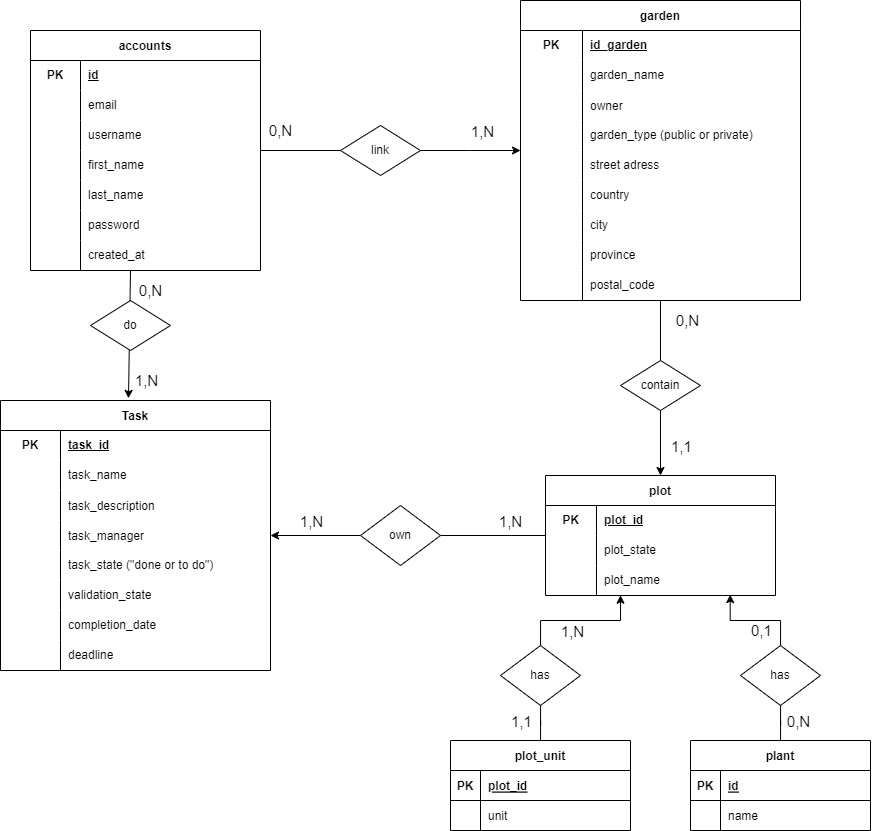
\includegraphics[width=1\textwidth]{img/Schema_entite_association_PPIIversion2.drawio.png}
    \caption{Schéma entité-association}
\end{figure}

Ce schéma respecte les contraintes logiques de cardinalités suivantes :

\begin{itemize}
    \item Une personne peut posséder/rejoindre un ou plusieurs jardins.
    \item Un jardin peut avoir plusieurs parcelles mais une parcelle est associée à un seul jardin.
    \item Une parcelle peut avoir plusieurs unités mais une unité est associée à une seule parcelle.
    \item Une parcelle peut avoir une plante et une plante peut être attribuée à plusieurs parcelles.
    \item Une personne peut effectuer plusieurs tâches et une tâche peut être effectuée par plusieurs personnes.
\end{itemize}

\subsubsection{Passage du modèle entité-association au relationnel}
A présent, nous allons transformer notre schéma entité-association en modèle relationnel en respectant les règles de la troisième forme
normale.

\begin{itemize}
    \item account(id, email, username, first\_name, last\_name, password, created\_at)
    \item garden(id\_garden, garden\_name, owner, manager, garden\_type, street\_adress, country, city, province, postal\_code)
    \item plot(plot\_id, garden\_id, plot\_state, plot\_name, plant)
    \item task(task\_id, plot\_id, task\_name, task\_description, task\_manager, task\_state, completion\_state, validation\_state, deadline)
    \item plot\_unit(plot\_id, x, y)
    \item plant(id, plant\_name, water\_need)
    \item do(account\_id, task\_id)
    \item link(account\_id, garden\_id)
\end{itemize}
\subsection{Implémentation de la base de données dans le backend de l'application}

\subsubsection{Création de la base de données}
En utilisant le système de gestion de base de données sqlite, nous avons créé notre base dans un fichier data.db avec le script
SQL sauvegardé dans un fichier nommé "creation table.sql". Ces deux fichiers sont dans le dossier backend/data du projet.


\subsubsection{Utilisation de SQLAlchemy}
SQLAlchemy est un ORM (Object-Relational Mapping) permettant de manipuler la base de données via des objets python. Les requêtes en
python sont ainsi "traduites" en SQL et la réponse reçue se présentera sous la forme d’un objet python avec lequel on peut interagir.
SQLAlchemy constitue donc un pont entre la base de données et notre application. Pour que l’ORM puisse fonctionner, il faut définir
des classes python qui correspondent aux tables de la base de données. Ces classes ont des attributs qui correspondent aux attributs
des tables. On appelle ça des modèles. Les modèles sont ensuite utilisés pour créer des requêtes SQL.

Les sessions de SQLAlchemy permettent de gérer les transactions SQL, autrement dit un ensemble de requêtes. Si l'une d'elles échoue,
l'ensemble de la transaction est annulée et aucune requête n'est communiquée à la base. L’avantage de ce système est la sécurité.

\newpage
\section{Serveur et client Web}
\subsection{Structure de l'application}
L'application est divisée en deux parties afin de pouvoir maitriser complètement le coté client, important pour la modélisation de jardins :
\begin{itemize}
    \item Le backend, qui est le coeur de l'application. C'est un serveur web flask. Celui-ci est décomposé en une multitudes de routes, retournant toutes du JSON. Il s'agit d'une API REST.
    \item Le frontend, qui est la partie visible de l'application. Il est entièrement réalisé avec Javascript, accompagné de la librairie React.js. Le frontend communique avec le backend via des requêtes HTTP, réalisées à l'aide de la librairie Axios.
\end{itemize}
\subsection{Fonctionnalités de l'application}
\subsubsection{Authentification}
L'application dispose d'un système d'authentification complet, afin de sécuriser l'ensemble, ainsi que pour personnaliser les fonctionnalités des utilisateurs. Cette authentification se déroule via des tokens JWT, générés par le serveur au moment de la connection, puis stockés dans les cookies du navigateur de l'utilisateur. Ces tokens sont ensuite utilisés pour vérifier l'identité de l'utilisateur, et ainsi lui permettre d'accéder aux routes protégées.
Cette authentification permet entre autres à l'utilisateur de créer, rejoindre des jardins, de les gérer, et de les partager en leur nom.

\subsubsection{Gestion de compte}
Un utilisateur authentifié dispose de plusieurs fonctionnalités afin de personnaliser et modifier son compte. Il peut ainsi modifier ses informations personnelles, telles que sa photo de profil et son nom.

\subsubsection{Gestion des jardins}
De nombreuses routes sont dédiées au management des jardins sur l'application. On peut en effet retrouver ces différentes opérations :
\begin{itemize}
    \item Récupérer un jardin, en fonction de son identifiant.
    \item Créer un jardin, en lui donnant un nom, une description, une adresse et en choisissant le type de jardin (privé ou public).
    \item Supprimer un jardin qu'un utilisateur a créé.
    \item Modifier les informations et les membres d'un jardin.
    \item Rejoindre un jardin.
\end{itemize}

\subsubsection{Carte interractive}
Afin de rendre plus accessible la fonctionnalité de rejoindre un jardin, il est également possible de le faire depuis une carte interractive, sur laquelle est listée l'intégralité des jardins publics, ainsi que ceux dont l'utilisateur est membre. Cette carte est réalisée à l'aide de la librairie Leaflet.

\subsubsection{Interractions avec le jardin}
Les utilisateurs membres de jardins peuvent interagir avec ceux-ci, en fonction de leurs permissions. On peut ainsi retrouver les fonctionnalités suivantes :
\begin{itemize}
    \item Créateur d'un jardin :
          \begin{itemize}
              \item Modéliser le jardin
              \item Gérer les utilisateurs du jardin
              \item Supprimer le jardin
          \end{itemize}
    \item Les membres et le créateur :
          \begin{itemize}
              \item Ajouter / supprimer des tâches à une parcelle
              \item Modifier les plantes des parcelles
          \end{itemize}
\end{itemize}
Ces fonctionnalités leur permettent donc de personnaliser au maximum leurs jardins.

\newpage
\section{Algorithme}
\subsection{Principe de l'algorithme}
Le problème à résoudre ici est de pouvoir alimenter en eau le potager de manière optimale. Pour cela, nous sommes partis sur l'idée de placer des arroseurs sur les parcelles du potager.
Cela permet de pouvoir arroser les plantes de manière optimale, en fonction de leurs besoins. Mais aussi, de pouvoir automatiser l'alimentation en eau du potager.
Ainsi le but de cet algorithme est donc de placer de manière optimale les arroseurs sur les parcelles pour en placer le moins possible.
\begin{figure}[H]
    \centering
    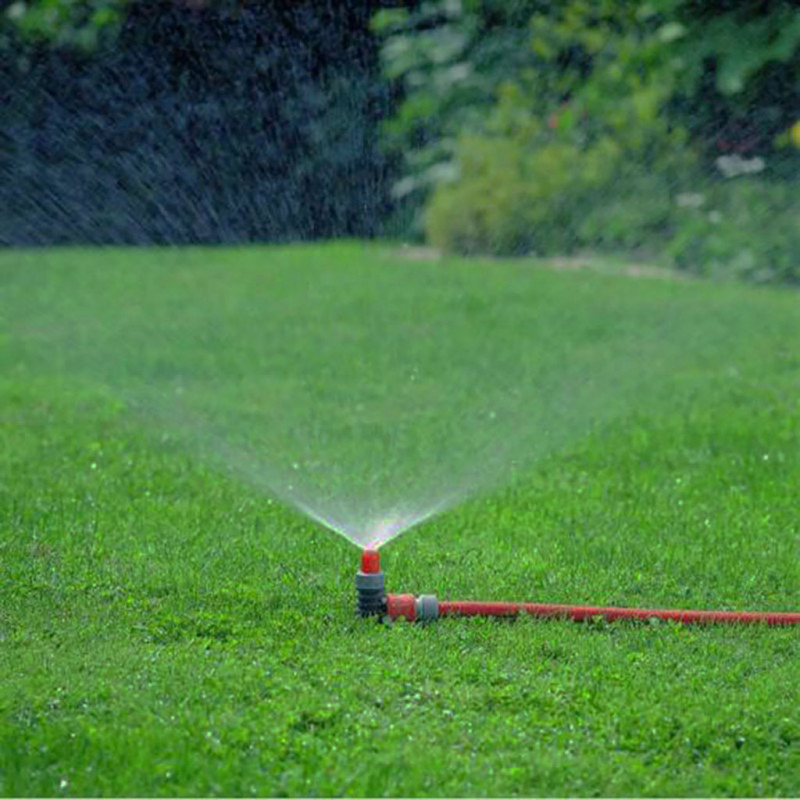
\includegraphics[width=0.4\textwidth]{img/arroseur-sur-pic.jpg}
    \caption{Arroseur sur pic}
\end{figure}

\subsection{Implémentation}
\subsubsection{Modélisation du problème}
Tout d'abord, nous avons modélisé le jardin sous la forme d'une matrice avec le module numpy pour avoir une matrice optimisée en python, c'était la façon la plus naturelle pour nous pour la représenter aussi bien en frontend qu'en algorithmique.
Ensuite, nous avons implémenté l'algorithme de placement des arroseurs. Pour cela, on a posé des contraintes :
\begin{itemize}
    \item Un arroseur alimente en eau la parcelle sur laquelle il est placé et les parcelles adjacentes.
    \item Une parcelle porte un poids qui correspond à la quantité d'eau dont elle a besoin.
    \item Un arroseur ne peut être placé que sur une parcelle.
    \item Un arroseur n'arrose qu'une fois une parcelle, ainsi une plante ayant un besoin de deux devra être arrosée par deux points d'eau différents et ainsi de suite.
\end{itemize}
Nous avons tout d'abord pensé à résoudre ce problème en développant un algorithme basé sur le backtracking sur le même principe que knapsack (problème des sacs à dos).
Cependant, le fait de devoir tester toutes les possibilités de placement des arroseurs rendait l'algorithme trop long à exécuter. Il n'était donc pas possible de l'utiliser pour un jardin de plus de 6x6 parcelles ce qui était plutôt limitant dans notre cas.
Nous avons ensuite tenté de placer les points d'eau sur les plantes qui avaient les plus forts besoins mais encore une fois, le placement n'était clairement pas optimisé et il fallait placer beaucoup de points d'eau pour arroser toutes les plantes surtout dans le cas où la matrice commencait à avoir une taille représentative d'un jardin.
Finalement, en prenant un autre point de vue sur le problème, il a été possible de le résoudre de manière très rapide.
Il suffit alors de se rendre compte que ce problème peut être traité sous la forme d'un problème mathématique, à travers un système d'équations contenant la position des points d'eau et les besoins des plantes.
Ainsi, la difficulté réside ici en la modélisation de ce problème en un système d'équations linéaires pour ensuite le résoudre sous la forme d'un modèle de programmation linéaire en nombres entiers.
Comment avons nous tout d'abord modélisé le potager en une matrice numpy ? :
\begin{itemize}
    \item Chaque parcelle est représentée par un nombre entier positif et correspond à des coordonnées (x,y) dans la matrice.
    \item Les parcelles vides sont représentées par un 0.
    \item Les parcelles contenant une plante sont représentées par un nombre entier positif correspondant au besoin en eau de la plante.
\end{itemize}
Prenons alors le cas d'un potager de taille 4x4 avec les besoins suivants :
\newline
\[M = \begin{bmatrix} 2 & 2 & 1 & 1 \\ 2 & 2 & 1 & 1 \\ 0 & 0 & 1 & 1 \\ 0 & 0 & 1 & 1 \end{bmatrix}\]
\newline Nous ferons allusion à la matrice M pour représenter le potager dans la suite pour plus de clarté et avoir un exemple concret.
\newline Nous avons donc ici un potager de taille 4x4 avec un ensemble de parcelles 2x2 contenant des plantes ayant un besoin en eau de 2. Puis un ensemble de parcelles 2x4 contenant des plantes ayant un besoin en eau de 1. Le reste de la matrice contient des zéros car les parcelles sont creusées mais ne contiennent pas de plantes, elles ont donc un besoin de 0.
\newline Nous allons maintenant modéliser ce problème en un système d'équations linéaires.
\subsubsection{Modélisation du problème en un système d'équations linéaires}
Pour cela, on part du constat que pour chaque parcelle de légumes, si on veut que cette parcelle voit son besoin en eau accompli, il faut que sa propre parcelle ou les parcelles adjacentes contiennent le nombre de points d'eau nécessaires pour assouvir son besoin. Ainsi, le poids de chaque parcelle correspond au nombre de points d'eau qu'il faut autour d'elle ou sur elle même.
Ainsi, cela constitue ce qu'on appelle une contrainte(*), on crée donc une équation pour chaque parcelle contenant une plante. Pour cela, on va écrire ce système d'équations linéaires sous la forme d'un produit matriciel.
\newline On pose alors X la matrice contenant l'ensemble des points d'eau que l'on peut placer, cela correspond au nombre d'éléments dans la matrice M :
\newline \[X = \begin{bmatrix} X_1 \\ X_2 \\ . \\ . \\ X_n \end{bmatrix}\]
\newline $X_i$ est égal à 1 si la case i est une source, et 0 sinon. On prend donc ici des valeurs binaires, soit on place un point d'eau, soit on en place pas.
\newline On pose ensuite la matrice C, qui est la matrice donnant la position, pour chaque parcelle, des sources d'eau :
\newline \[C = \begin{bmatrix} c_{1,1} & c_{1,2} & . & . & c_{1,n} \\ c_{2,1} & c_{2,2} & . & . & c_{2,n} \\ . & . & . & . & . \\ . & . & . & . & . \\ c_{n,1} & c_{n,2} & . & . & c_{n,n} \end{bmatrix}\]
\newline $c_{i,j}$ est égal à 1 si la case j est adjacente à la case i, et 0 sinon.
\newline On pose ensuite la matrice B, qui est la matrice donnant le besoin en eau pour chaque parcelle des sources d'eau :
\newline \[B = \begin{bmatrix} b_1 \\ b_2 \\ . \\ . \\ b_n \end{bmatrix}\]
\newline $b_i$ est égal au besoin en eau de la parcelle i.
\newline Ainsi, à l'aide de la contrainte que l'on se fixe ici (*), on peut poser alors notre système d'équations linéaires sous la forme :
\newline \begin{equation} C \cdot X = B \end{equation}
\newline
\newline On a alors un système d'équations détaillé de cette forme :
\newline
\begin{equation}
    \begin{aligned}
         & c_{1,1}x_1+c_{1,2}x_2+...+c_{1,n^2}x_{n^2} \ge b_1 \ , x_{n^2} \in \{0,1\}           \\
         & c_{2,1}x_1+c_{2,2}x_2+...+c_{2,n^2}x_{n^2} \ge b_2 \ , x_{n^2} \in \{0,1\}           \\
         & ...                                                                                  \\
         & c_{n^2,1}x_1+c_{n^2,2}x_2+...+c_{n^2,n^2}x_{n^2} \ge b_{n^2} \ , x_{n^2} \in \{0,1\}
    \end{aligned}
\end{equation}
\newline
\newline où $c_{i,j}$ indique si le point d'eau peut être placé pour augmenter son besoin ou pas.
\newline On peut alors résoudre ce système d'équations linéaires pour trouver le nombre de points d'eau à placer pour chaque parcelle.
\newline Montrons maintenant concrètement ce qu'il se passe au travers de la matrice M constituant un exemple de potager.
\newline Tout d'abord, voici la matrice C de l'explication précédente :
\[C = \begin{bmatrix} 
1 & 1 & 0 & 0 & 1 & 1 & 0 & 0 & 0 & 0 & 0 & 0 & 0 & 0 & 0 & 0 \\ 
1 & 1 & 1 & 0 & 1 & 1 & 1 & 0 & 0 & 0 & 0 & 0 & 0 & 0 & 0 & 0 \\ 
0 & 1 & 1 & 1 & 0 & 1 & 1 & 1 & 0 & 0 & 0 & 0 & 0 & 0 & 0 & 0 \\ 
0 & 0 & 1 & 1 & 0 & 0 & 1 & 1 & 0 & 0 & 0 & 0 & 0 & 0 & 0 & 0 \\ 
1 & 1 & 0 & 0 & 1 & 1 & 0 & 0 & 1 & 1 & 0 & 0 & 0 & 0 & 0 & 0 \\ 
1 & 1 & 1 & 0 & 1 & 1 & 1 & 0 & 1 & 1 & 1 & 0 & 0 & 0 & 0 & 0 \\ 
0 & 1 & 1 & 1 & 0 & 1 & 1 & 1 & 0 & 1 & 1 & 1 & 0 & 0 & 0 & 0 \\ 
0 & 0 & 1 & 1 & 0 & 0 & 1 & 1 & 0 & 0 & 1 & 1 & 0 & 0 & 0 & 0 \\ 
0 & 0 & 0 & 0 & 0 & 1 & 1 & 1 & 0 & 1 & 1 & 1 & 0 & 1 & 1 & 1 \\ 
0 & 0 & 0 & 0 & 0 & 0 & 1 & 1 & 0 & 0 & 1 & 1 & 0 & 0 & 1 & 1 \\ 
0 & 0 & 0 & 0 & 0 & 0 & 0 & 0 & 0 & 1 & 1 & 1 & 0 & 1 & 1 & 1 \\ 
0 & 0 & 0 & 0 & 0 & 0 & 0 & 0 & 0 & 0 & 1 & 1 & 0 & 0 & 1 & 1
\end{bmatrix}\]
\newline
Ensuite on a la matrice B correspondante au besoin des plantes dans le potager :
\newline
\[B = \begin{bmatrix} 2 & 2 & 1 & 1 & 2 & 2 & 1 & 1 & 1 & 1 & 1 & 1 \end{bmatrix}\]
\newline
On obtient alors le système d'équations linéaires suivante :
\newline
\begin{equation}
    \begin{aligned}
         & x_1+x_2+x_5+x_6 \ge 2 \ , x_{n^2} \in \{0,1\}                                       \\
         & x_1+x_2+x_3+x_5+x_6+x_7 \ge 2 \ , x_{n^2} \in \{0,1\}                               \\
         & x_2+x_3+x_4+x_6+x_7+x_8 \ge 1 \ , x_{n^2} \in \{0,1\}                               \\
         & x_3+x_4+x_7+x_8 \ge 1 \ , x_{n^2} \in \{0,1\}                                       \\
         & x_1+x_2+x_5+x_6+x_1+x_2+x_9+x_{10} \ge 2 \ , x_{n^2} \in \{0,1\}                    \\
         & x_1+x_2+x_3+x_5+x_6+x_7+x_9+x_{10}+x_{11} \ge 2 \ , x_{n^2} \in \{0,1\}             \\
         & x_2+x_3+x_4+x_5+x_6+x_7+x_8+x_{10}+x_{11}+x_{12} \ge 1 \ , x_{n^2} \in \{0,1\}      \\
         & x_3+x_4+x_7+x_8+x_{11}+x_{12} \ge 1 \ , x_{n^2} \in \{0,1\}                         \\
         & x_6+x_7+x_8+x_{10}+x_{11}+x_{12}+x_{14}+x_{15}+x_{16} \ge 1 \ , x_{n^2} \in \{0,1\} \\
         & x_7+x_8+x_{11}+x_{12}+x_{15}+x_{16} \ge 1 \ , x_{n^2} \in \{0,1\}                   \\
         & x_{10}+x_{11}+x_{12}+x_{14}+x_{15}+x_{16} \ge 1 \ , x_{n^2} \in \{0,1\}             \\
         & x_{11}+x_{12}+x_{15}+x_{16} \ge 1 \ , x_{n^2} \in \{0,1\}                           \\
    \end{aligned}
\end{equation}
\newline
Ainsi trouver les $x_i$ qui vérifient ce système d'équations est une solution pour placer les points d'eau.
Mais il existe de multiples solutions à ce problème, alors comment faire pour avoir la plus optimale ?
\subsubsection{Optimisation du système d'équations linéaires}
Pour cela, on va utiliser la méthode de la programmation linéaire. On va donc chercher à minimiser le nombre de points d'eau à placer pour que chaque parcelle ait son besoin en eau accompli. L'astuce ici réside dans le fait de chercher à minimiser la somme des points d'eau à placer, car $x_{i,j}$ correspond à des valeurs binaires, soit 0 soit 1.
\newline On pose alors la fonction objectif qui est la somme des points d'eau à placer :
\newline
\newline \begin{equation} f(X) = \sum_{i=1}^{n^2} x_i \end{equation}
\newline
\newline On peut donc écrire notre problème sous la forme :
\newline
\newline \begin{equation} \min (f(X)) \end{equation}
\newline
\newline Il faut savoir qu'en programmation linéaire, il faut fixer un objectif à atteindre car c'est le but de l'optimisation linéaire, ici, cela sera de minimiser le plus possible la somme des points d'eau résultante.
\newline Ainsi en fournissant ces matrices, la contrainte étant le système d'équations linéaires qui découle du produit matriciel entre la matrice des variables (points d'eau), la matrice C qui est leur proximité avec chaque parcelle et la matrice B le besoin en eau de chaque parcelle. On peut alors résoudre ce problème en programmation linéaire à l'aide ici du module Gurobipy de Python en fixant l'objectif décrit ci-dessus.
\newline On obtient finalement la position des points d'eau à placer dans le jardin, et grâce au modèle mathématique qui repose sur la programmation linéaire, on peut être sûr que la solution fournie est optimale.
\newline Ainsi, dans notre exemple, on obtient :
\newline
\[ B = \begin{bmatrix} 0 & 1 & 0 & 0 \\ 0 & 1 & 0 & 1 \\ 0 & 0 & 1 & 0 \\ 0 & 0 & 0 & 0 \end{bmatrix}\]
\newline
Et on observera alors que, effectivement, dans notre cas, le nombre de points d'eau ne peut être inférieur à 4, et il nous propose bien le positionnement de 4 points d'eau.
On a donc bien trouvé la solution optimale à notre problème ainsi qu'un placement possible (car il existe parfois d'autres placements de ces points qui vérifient aussi la solution mais cela n'a pas d'intêret ici).
\subsection{Analyse en complexité}
Si on compare par rapport à notre première version :
\newline
\newline Le script utilise la technique de backtracking pour trouver la solution optimale, c'est-à-dire le minimum de points d'eau nécessaires pour arroser toutes les plantes dans le potager. Pour chaque case (i, j) du potager, le script explore deux possibilités : mettre un point d'eau ou ne pas en mettre. Cela signifie que pour chaque case du potager, le script fait un appel récursif, ce qui multiplie par deux le nombre d'appels récursifs à chaque itération.
De plus, la fonction "backtrack" parcourt chaque case du potager (nm cases au total), ce qui multiplie encore une fois le nombre total d'appels récursifs par nm.
\newline Ainsi, la complexité de ce script est en : \[\mathcal{O}(2^{(m*n)}*m*n) = \mathcal{O}(3^{(m*n)})\]
\newline Dans notre second algorithme :
\newline L'algorithme utilise l'optimiseur Gurobi pour résoudre un modèle de programmation linéaire en nombres entiers. La complexité de cet algorithme dépend de la complexité de l'optimiseur Gurobi.
La première partie de l'algorithme, qui construit les matrices C et B à partir de la matrice M, est en temps \[\mathcal{O}(n^2)\] Où n est le nombre d'élément dans la matrice du potager, car pour créer la matrice C, on crée pour chaque élément parcouru dans la matrice, on crée une liste de taille n, on a donc une complexité en : \[\mathcal{O}(n^2)\] Contrairement à la construction de la matrice B qui est en : \[\mathcal{O}(n)\]
L'optimisation elle-même est généralement considérée comme étant en : \[\mathcal{O}(n^3)\] Où n est le nombre de variables.
Dans l'ensemble, on peut considérer que la complexité globale de cet algorithme est de l'ordre de : \[\mathcal{O}(n^3)\] Où n est le nombre d'éléments de la matrice du potager.
\subsection{Analyse de performance}
Ici, nous allons en profiter pour comparer nos deux algorithmes avec des matrices carrées de taille n, dont la taille va augmenter de 1 à chaque fois. Voici les graphes résultants de ses tests :
\begin{figure}[H]
    \centering
    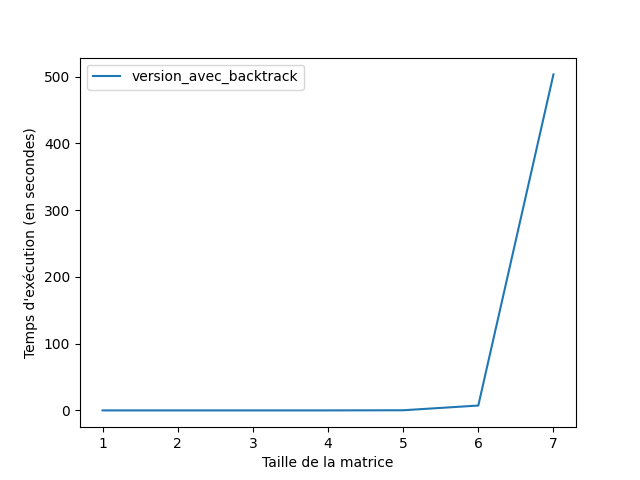
\includegraphics[width=0.5\textwidth]{img/backtrack.png}
    \caption{Courbe de performance de l'algorithme de backtracking}\label{fig:figure}
\end{figure}
\begin{figure}[H]
    \centering
    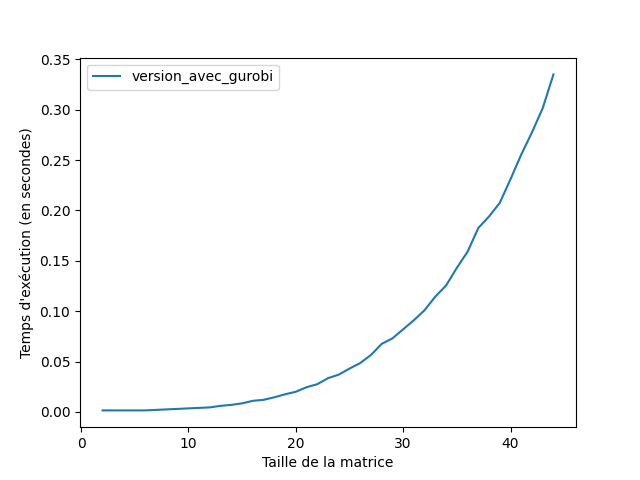
\includegraphics[width=0.5\textwidth]{img/gurobi.png}
    \caption{Courbe de performance de l'algorithme de programmation linéaire}\label{fig:figure2}
\end{figure}
\begin{figure}[H]
    \centering
    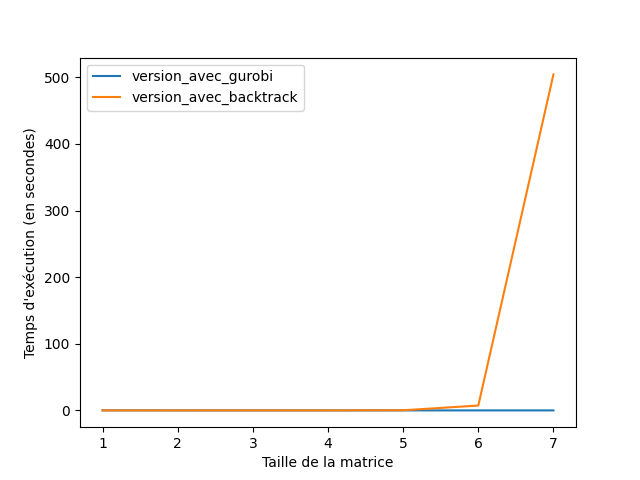
\includegraphics[width=0.5\textwidth]{img/comparaison_algo.png}
    \caption{Comparaison des deux algorithmes}\label{fig:figure3}
\end{figure}
On voit que très clairement, la version avec le module Gurobipy est beaucoup plus rapide que la version avec backtracking, et cela est logique en vu de la complexité de ces deux algorithmes explicités précédemment.
On remarque surtout que, dans le cas du backtracking, la complexité croit très vite et que pour des matrices de taille 7, le temps d'exécution est déjà très long à tel point qu'il est déjà beaucoup trop long pour une matrice 8x8. Alors que pour la version avec gurobi, la complexité est beaucoup plus stable, et on peut même voir que pour des matrices de taille 45x45, le temps d'exécution est toujours inférieur à 0.4 secondes. Ce qui en fait notre algorithme préféré pour résoudre ce problème, surtout qu'il est le seul à pouvoir traiter notre potager de taille 12x12 en un temps plus que raisonnable.
\newpage
\section{Gestion de projet}
\subsection{Équipe de projet}
Ce projet est un projet local réalisé en groupe de 4 personnes~:
\begin{itemize}
    \item Alexis MARCEL
    \item Lucas LAURENT
    \item Noé STEINER
    \item Mathias AURAND-AUGIER
\end{itemize}
Le comité de pilotage est constitué de~:
\begin{itemize}
    \item Anne-Claire HEURTEL
    \item Olivier FESTOR
    \item Gérald OSTER
\end{itemize}
Ces personnes constituent les parties prenantes de notre projet ainsi que les acteurs influents sur le livrables.
\begin{figure}[H]
    \centering
    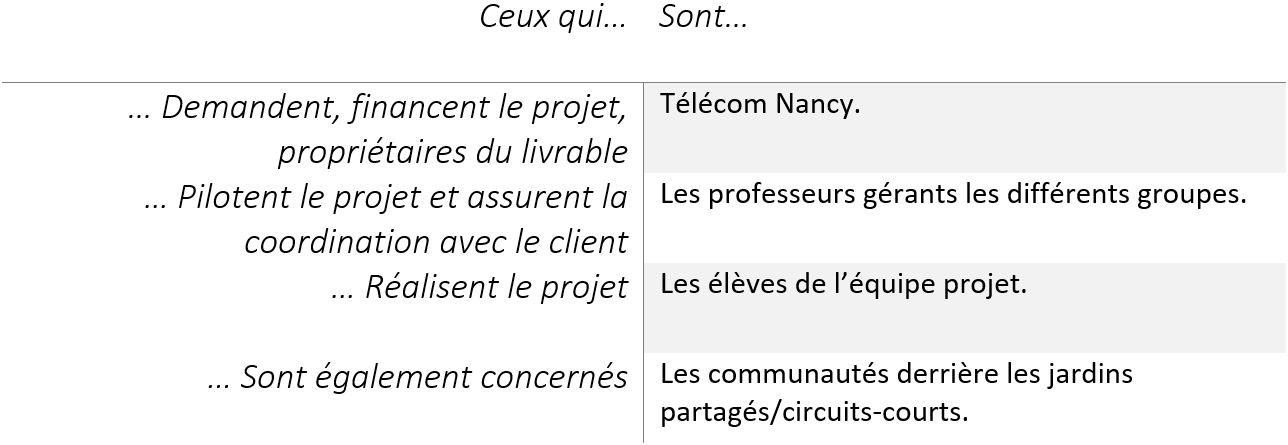
\includegraphics[width=0.75\textwidth]{img/parties_prenantes.png}
    \caption{Parties prenantes}
\end{figure}
\subsection{Organisation au sein de l’équipe projet}
Nous avons réalisé plusieurs réunions, en présentiel dans les locaux de Télécom Nancy mais la plupart de notre collaboration a eu lieu sur Discord. Ces réunions nous ont permis de mettre en commun nos avancées régulièrement, de partager nos connaissances sur des problématiques et de nous organiser de manière optimale.
En plus des réunions d'avancement règulières, nous avons également réalisé des réunions techniques afin de résoudre un problème ou bien de réflechir à la conception.
Les comptes rendus des réunions réalisées sont présents dans l’\hyperlink{annexe1}{Annexe 1}.

De plus, dès le début de notre projet nous avons mis en place un projet Trello. Trello est une application permettant d’organiser facilement un projet en reposant sur une organisation en planches listant des cartes, chacune représentant des tâches. Ces tâches peuvent ensuite être déplacées permettant de découper notre projet en plusieurs jalons dynamiquement.
\begin{figure}[H]
    \centering
    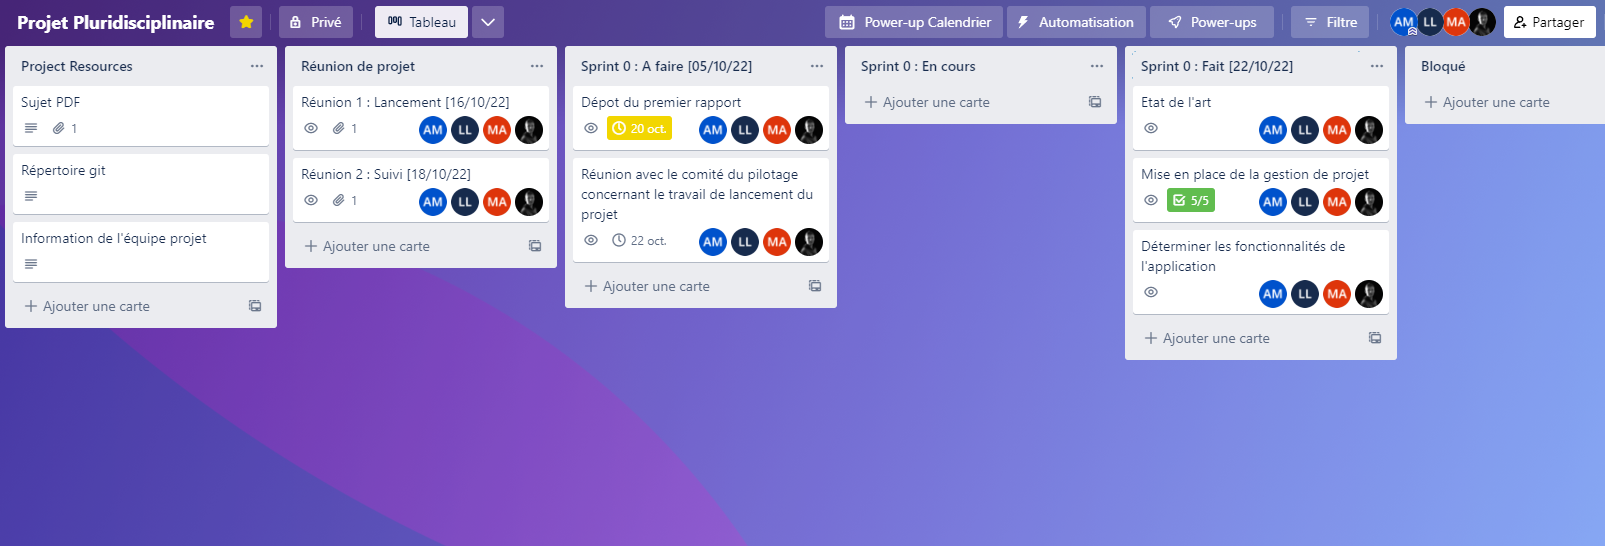
\includegraphics[width=0.75\textwidth]{img/trello.png}
    \caption{Organisation Trello}
\end{figure}

Ensuite, nous avons utilisé GitLab pour gérer les différentes versions du développement de notre application, ainsi que les différentes branches nous permettant de travailler simultanément sans conflit.

Enfin, la rédaction des differents comptes rendu de réunion et des rapports ont été rédigé en \LaTeX.

\subsection{Objectifs SMART}
La méthode SMART que l'on rappelle ci-dessous nous a permis de définir nos différents objectifs :

\begin{figure}[H]
    \centering
    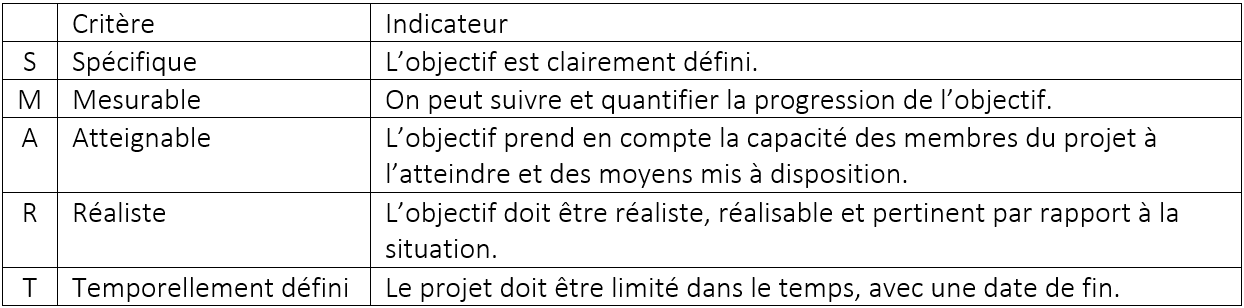
\includegraphics[width=1\textwidth]{img/SMART.png}
    \caption{Objectifs SMART}
\end{figure}

\subsection{Matrice des objectifs}
Nous avons conçu, à l'aide de la méthode SMART, la matrice des objectifs suivante :

\begin{figure}[H]
    \centering
    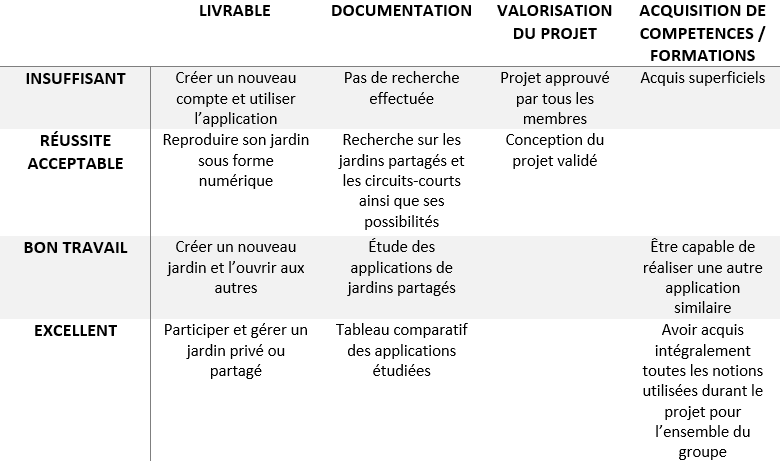
\includegraphics[width=1\textwidth]{img/matrice_des_objectifs.png}
    \caption{Matrice des objectifs}
\end{figure}

\subsection{Triangle qualité-cout-délai}
Afin d’établir des objectifs cohérents, et réalisables dans les délais, nous avons réalisé le triangle qualité-coût-délai. On remarque ainsi, les délais étant courts, que nous avons tout intérêt à ne pas se fixer des objectifs trop ambitieux sous peine de devoir renoncer à certaines fonctionnalités et de ne pas rendre le livrable annoncé initialement.

\begin{figure}[H]
    \centering
    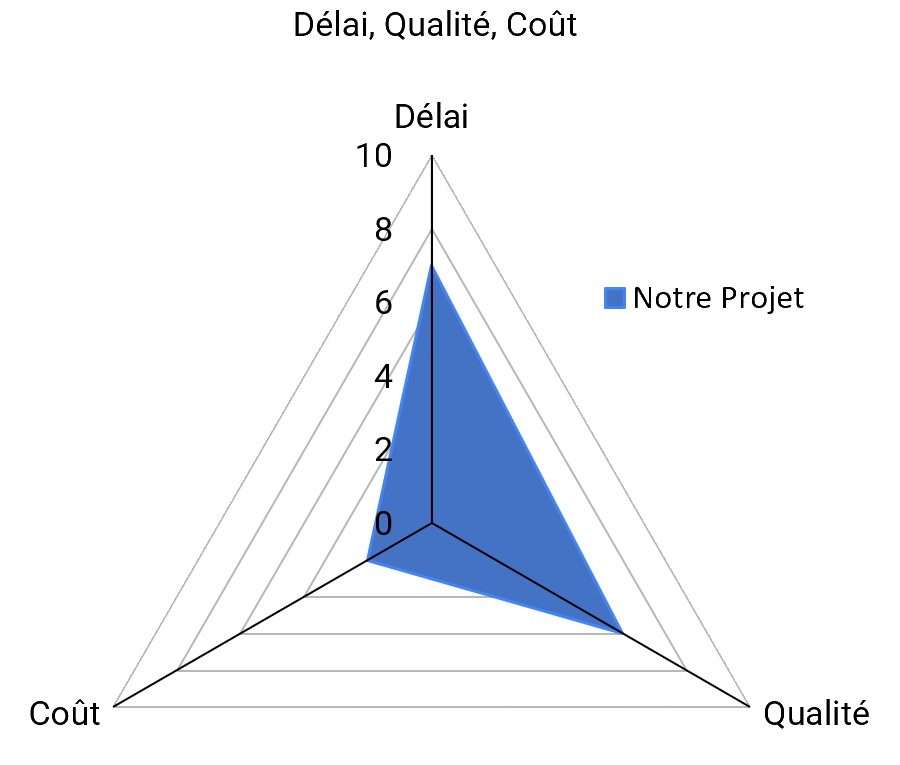
\includegraphics[width=0.5\textwidth]{img/triangle_QCD.png}
    \caption{Triangle DQC}
\end{figure}

\subsection{Matrice SWOT}
Afin d’avoir une vision plus globale de nos ressources et des facteurs internes et externes agissant sur le projet, nous avons ensuite réalisé la matrice SWOT (Strengths, Weaknesses, Opportunities, Threats) de notre projet.

\begin{figure}[H]
    \centering
    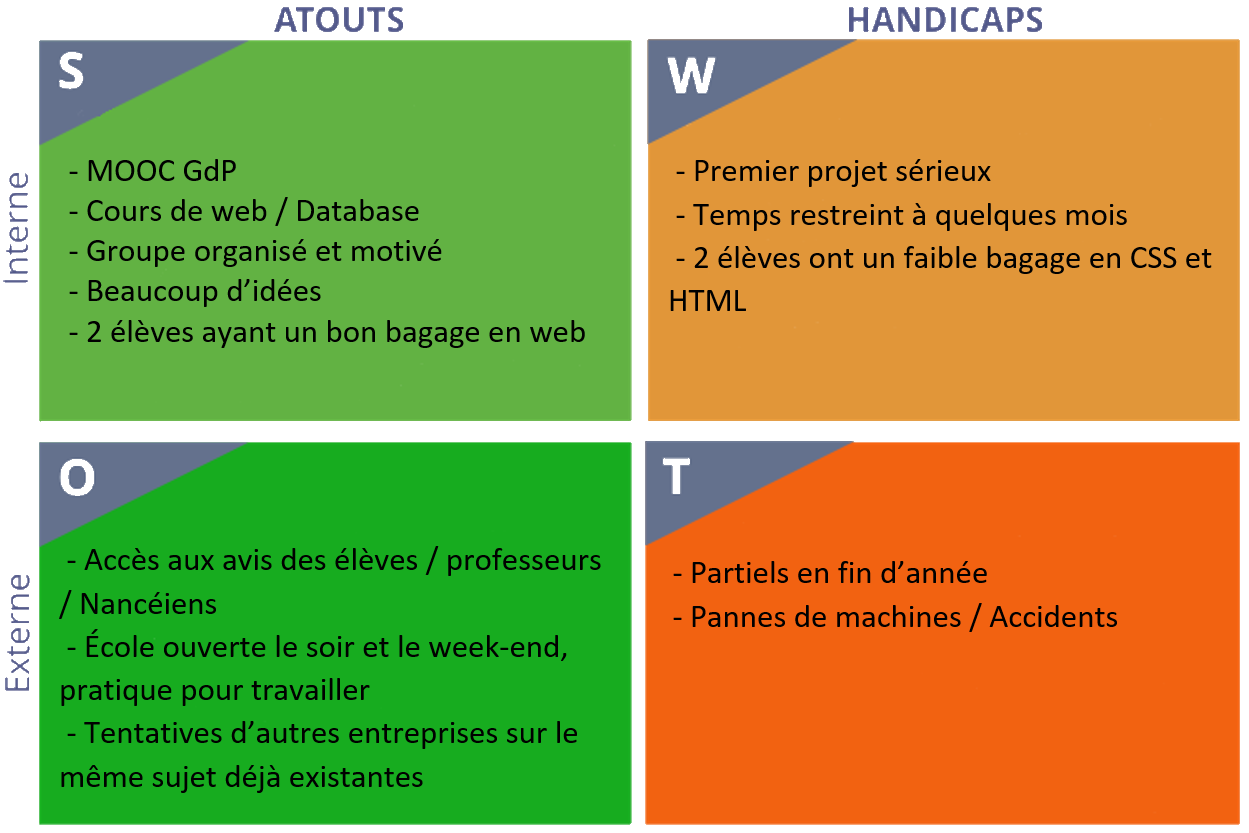
\includegraphics[width=0.75\textwidth]{img/SWOT.png}
    \caption{Matrice SWOT}
\end{figure}

On peut ainsi remarquer que notre projet présente de nombreux points forts notamment grâce aux connaissances acquises lors des cours de Télécom Nancy mais également de part l’expérience forte de deux des membres de l’équipe projet qui ont déjà réalisé des applications similaires.  Cependant, plusieurs facteurs internes constituent nos faiblesses notamment les courts délais qui nous obligent à être concis et efficaces dans notre travail, ou encore le faible bagage informatique de deux des membres de l’équipe. Néanmoins, ces lacunes constituent pour eux l’opportunité d’apprendre, et de progresser avec l’aide des membres expérimentés de l’équipe.

De plus, nous devons anticiper les charges de travail dans le cadre de notre formation à Télécom Nancy qui s'avèrent être plus élevées en décembre lors des partiels de fin d'année. Nous allons donc devoir prendre cela en compte dans notre gestion des tâches.

\subsection{Profil de projet}
Afin d’avoir une vision plus globale sur notre projet, nous avons également réalisé le profil du projet (le budget étant égal à 0, nous avons choisi de ne pas le représenter dans notre profil). On remarque que, du fait des nombreuses fonctionnalités que nous avons l’intention d’implémenter dans notre application, que notre projet est de taille moyenne mais de complexité élevée.

Cependant, les enjeux du projet ne sont pas très importants (en dehors de la note finale qui compte dans notre moyenne) car l'échec du projet n'engendrera pas la chute d'une organisation et le budget est négligeable.

De plus, au vu de l’état de l’art établi, l’innovation du projet est importante puisque nous avons choisi de combiner différentes fonctionnalités existantes de plusieurs applications et d’en rajouter de nouvelles.

\begin{figure}[H]
    \centering
    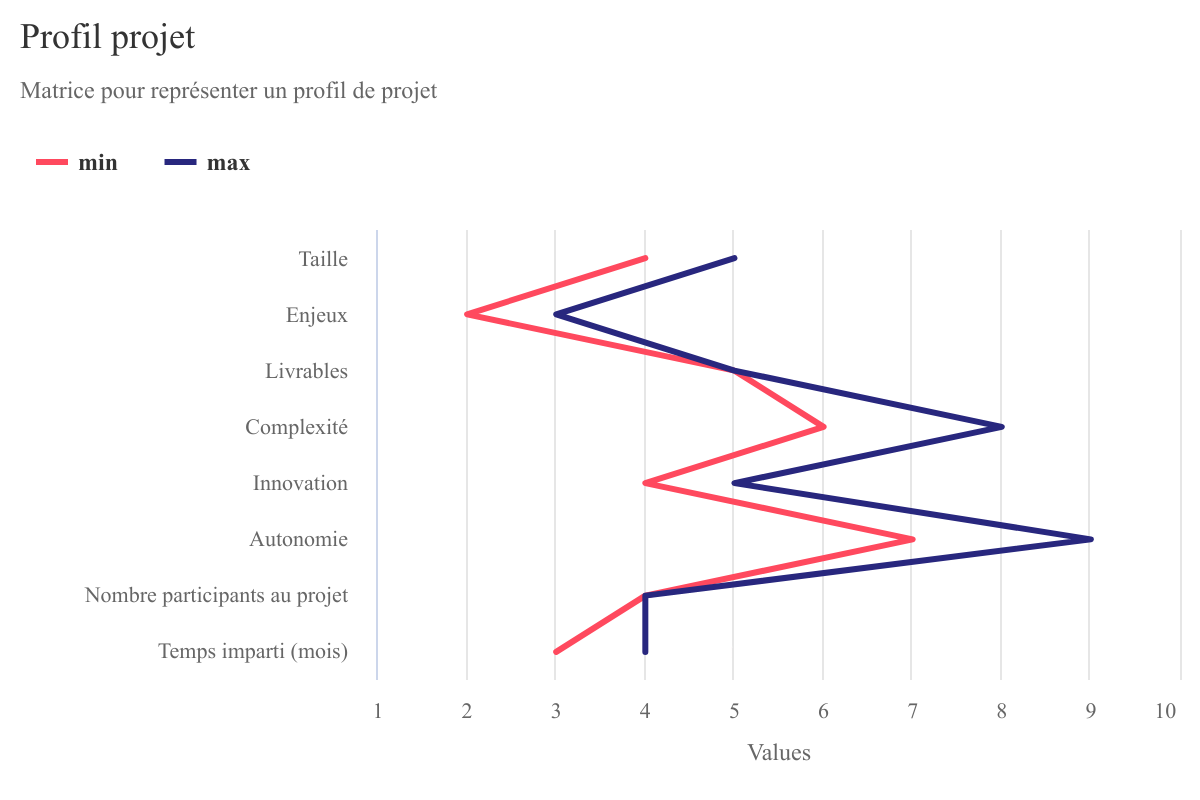
\includegraphics[width=0.75\textwidth]{img/profil_projet.png}
    \caption{Profil du projet}
\end{figure}

\subsection{WBS~: comment concrétiser l’application}
Ceci étant fait, nous avons maintenant choisi de détailler les lots de travail à effectuer pour fabriquer notre application. Nous avons ainsi réalisé le WBS (Work Breakdown Structure) de notre application~: il apparait ainsi les grandes étapes de notre projet que sont~: définition du cadre de l’application, développement des fonctionnalités de l’application et écriture du rapport.
\begin{figure}[H]
    \centering
    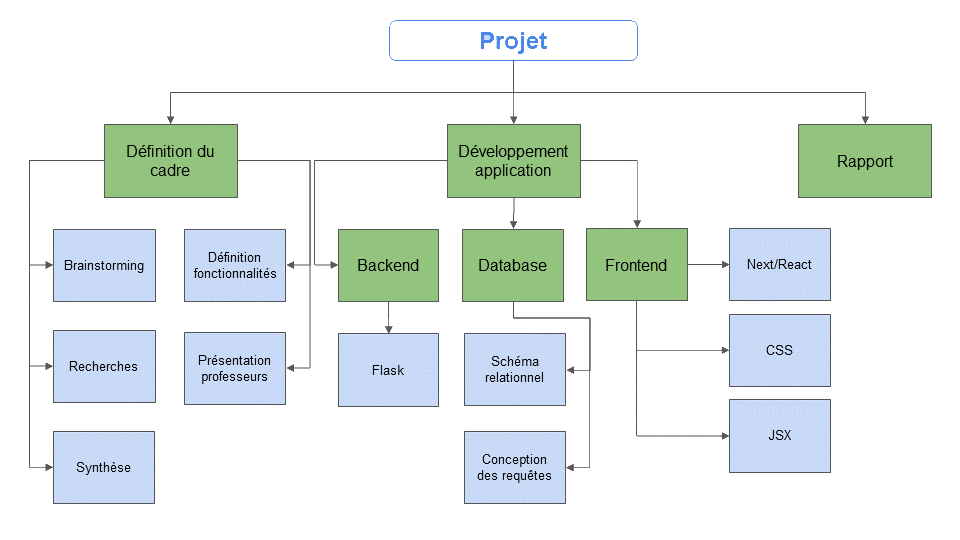
\includegraphics[width=1\textwidth]{img/WBS.png}
    \caption{WBS}
\end{figure}

\subsection{Diagramme de Gantt~: planification}
Maintenant que nous avons un détail des lots de travail qui constituent notre application, il faut maintenant les mettre en relation pour créer un planning efficace où chaque tâche est effectuée dans l’ordre.
\begin{figure}[H]
    \centering
    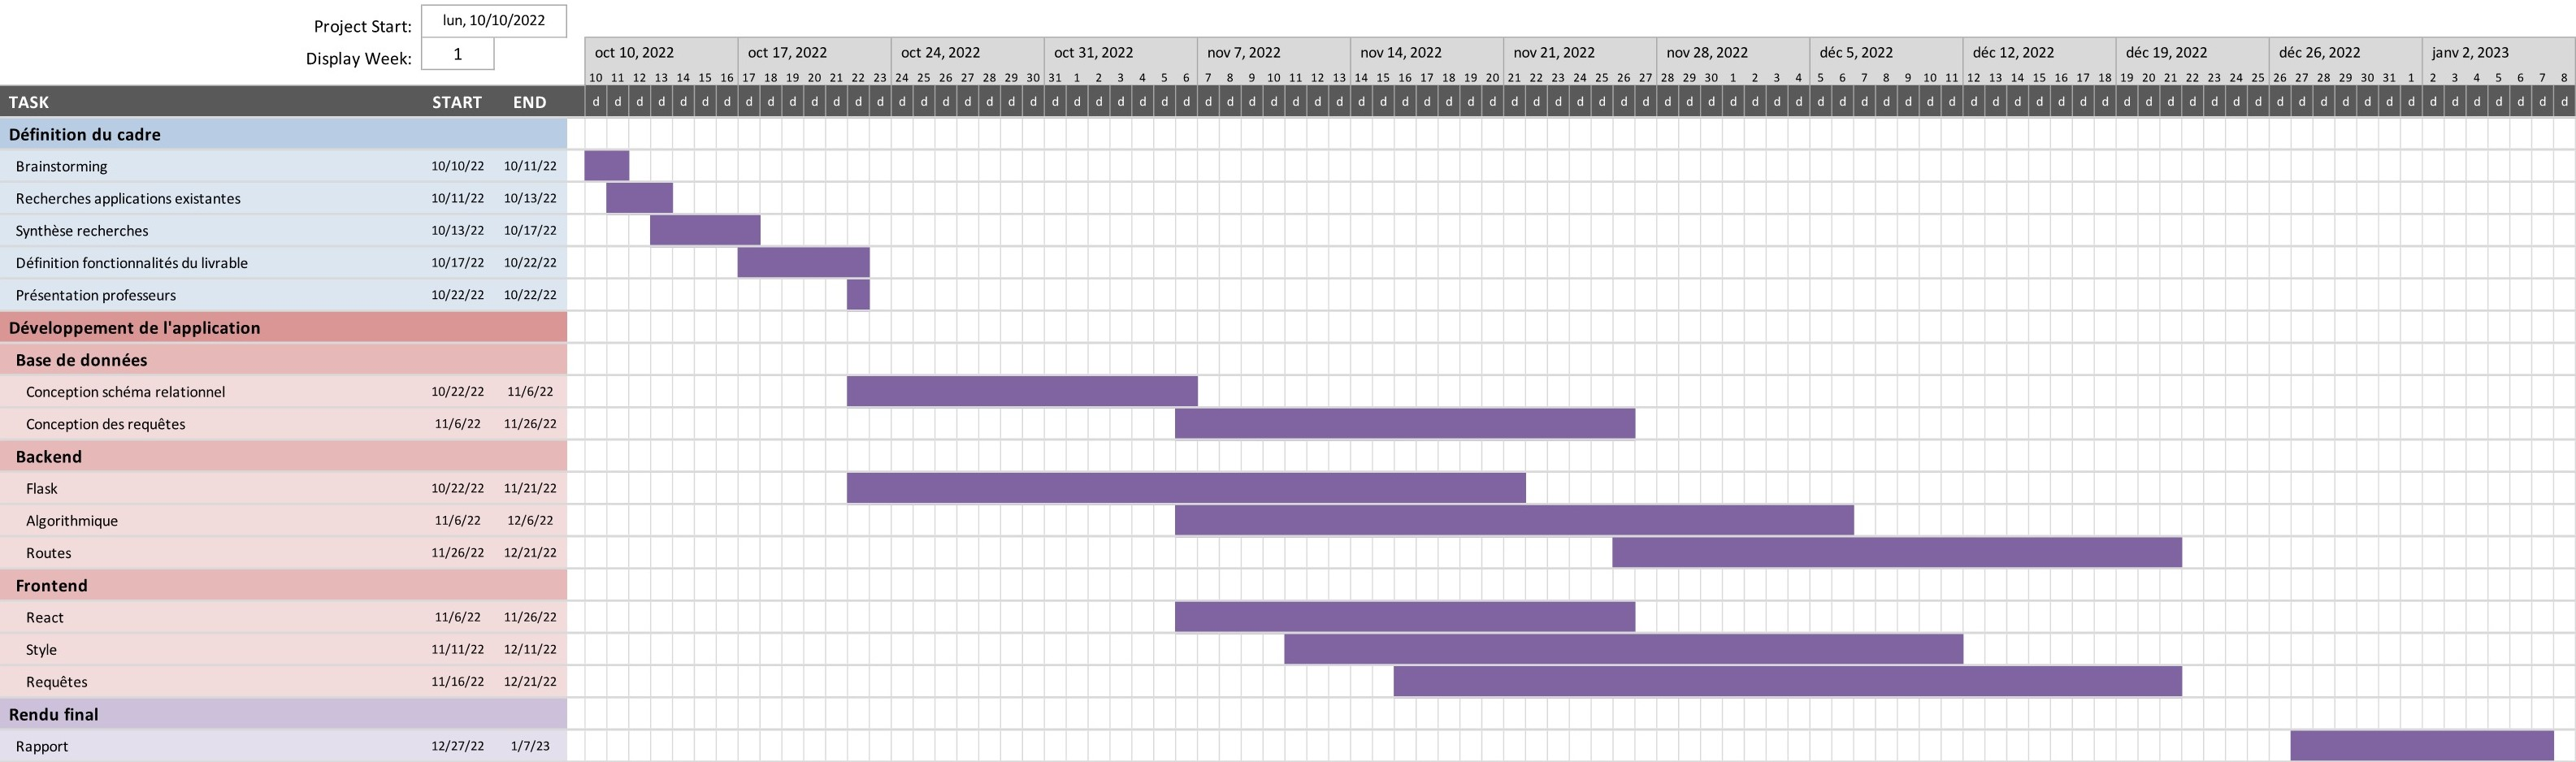
\includegraphics[width=1\textwidth]{img/gantt.png}
    \caption{Diagramme de GANTT}
\end{figure}
Ce diagramme est une première version générale des tâches à effectuer, il sera modifié et détaillé davantage une fois la conception et les maquettes du projet réalisées.

\subsection{Matrice RACI}
Maintenant que toutes les étapes sont planifiées, nous devons répartir le travail entre les membres de l’équipe. On utilise ainsi une matrice RACI synthétisant les rôles de chacun.

\begin{figure}[H]
    \centering
    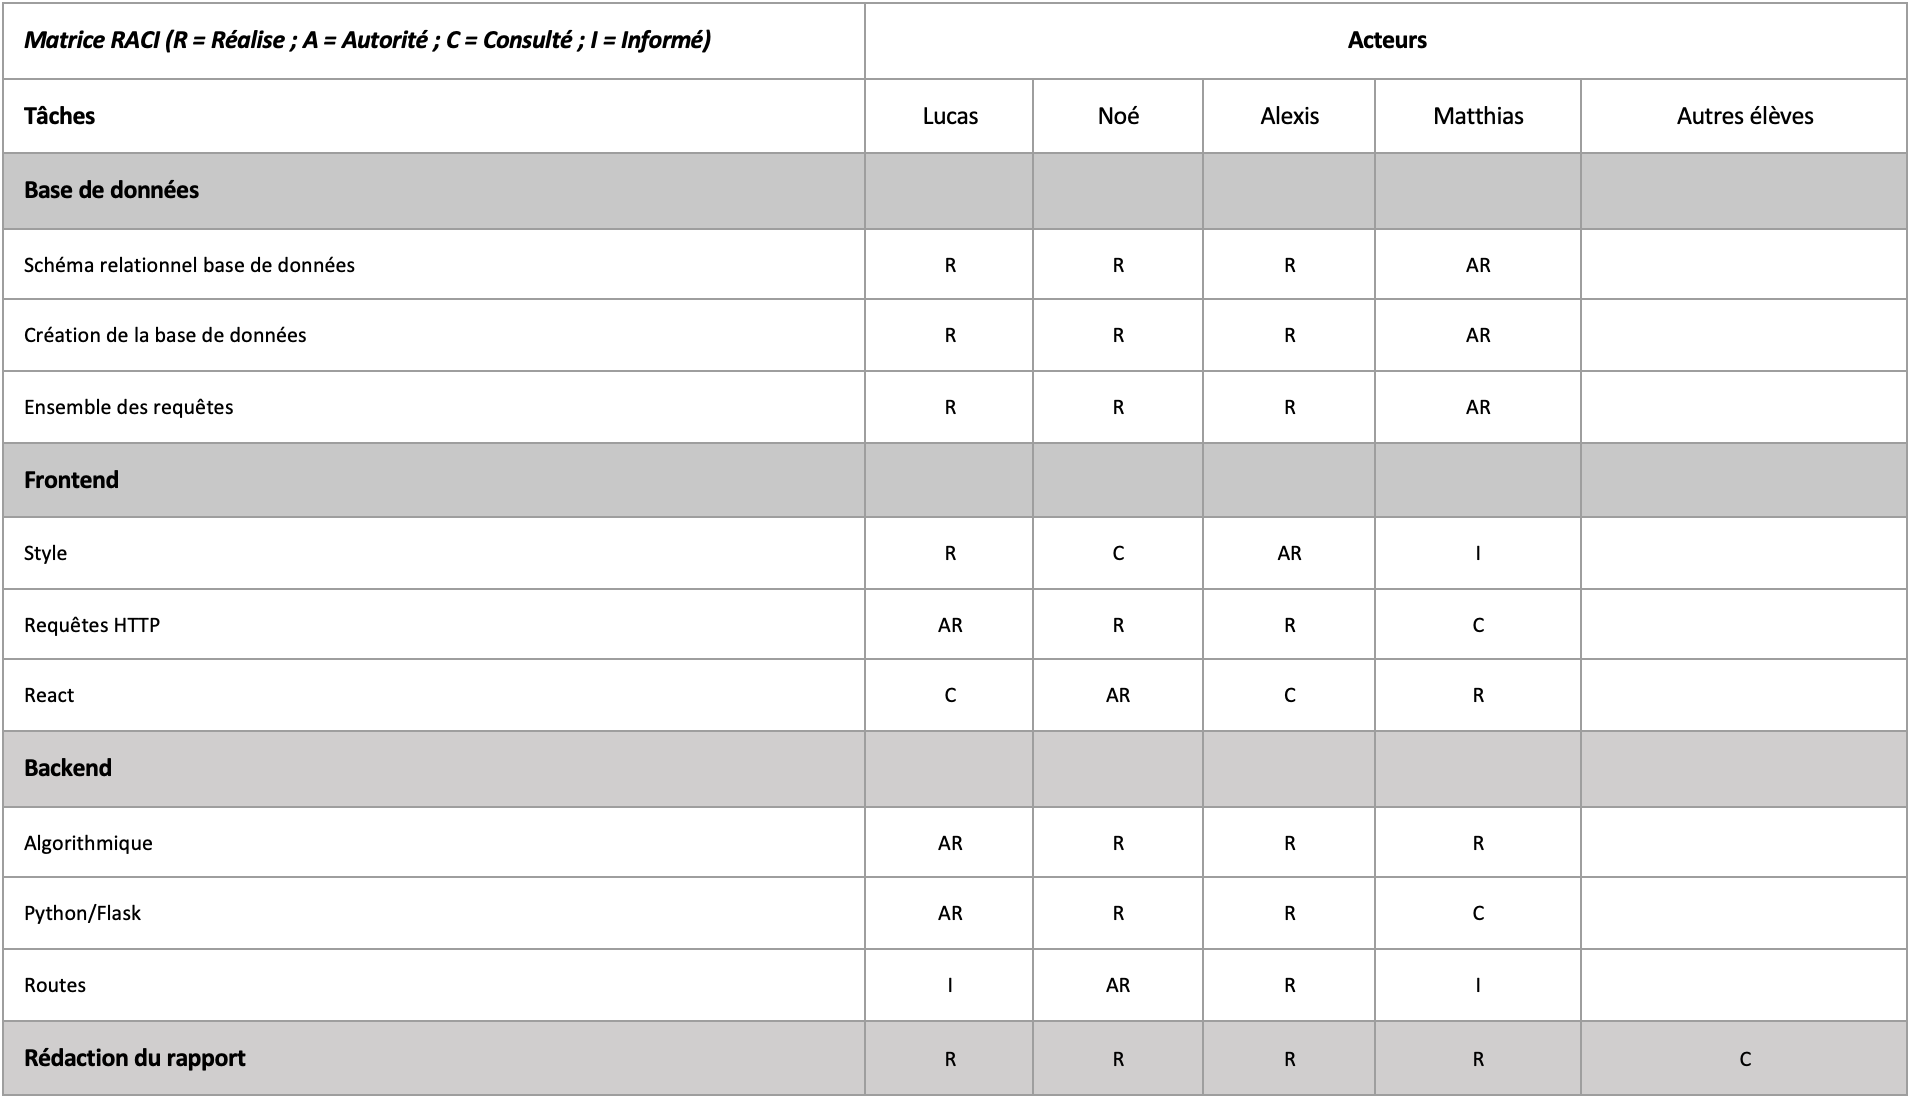
\includegraphics[width=1\textwidth]{img/RACI.png}
    \caption{Matrice RACI}
\end{figure}

\subsection{Gestion des risques}
Nous avons également pensé à prévoir une partie des risques pouvant se dresser sur notre route, les risques les plus classiques étant
la gestion du temps et le manque de compréhension de certaines personnes de l'équipe.
\begin{figure}[H]
    \centering
    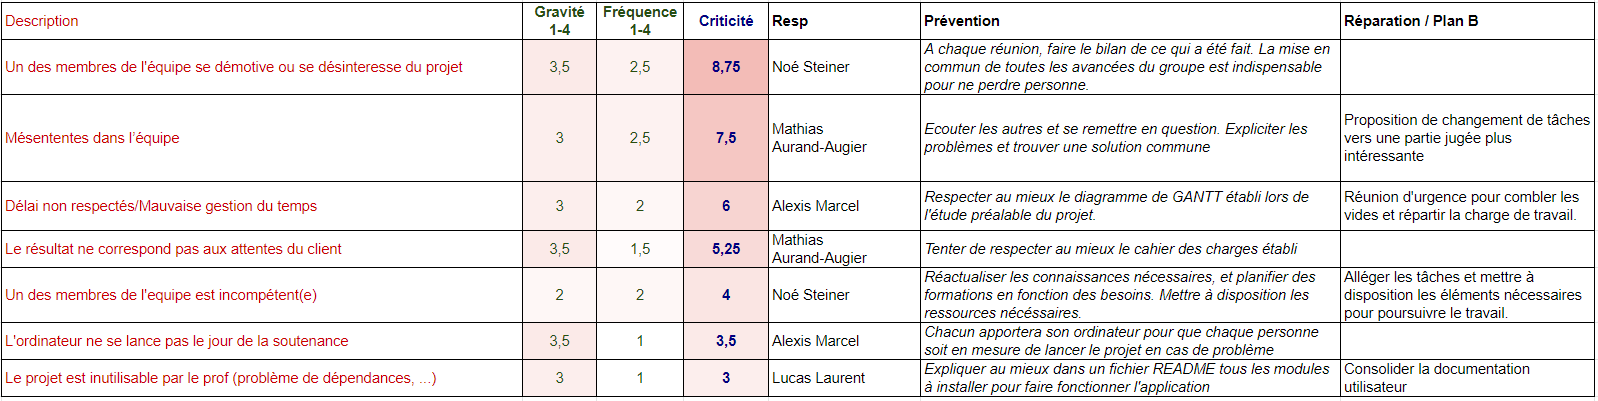
\includegraphics[width=1\textwidth]{img/Plan_gestion_risque.png}
    \caption{Plan de gestion des risques}
\end{figure}

\section{Conclusion}
Ce projet nous a permis de réaliser un projet de A à Z, de la conception à la réalisation. Nous avons pu mettre en pratique les connaissances acquises en cours et nous avons pu nous familiariser avec les outils de gestion de projet. Nous avons également pu nous rendre compte de la difficulté de la gestion de projet et de la nécessité de bien planifier son travail.
Nous avons réalisé la totalité des fonctionnalités et des éléments prévus lors de la phase de conception, ce qui nous permet de qualifier notre travail d'excellent selon notre matrice des objectifs.
Ce travail a également été l'occasion de découvrir de nouvelles technologies, comme les librairies React, Gurobipy et SQLAlchemy, mais également de découvrir de nouvelles méthodes de résolution de problème, via notre algorithme d'optimisation de l'arrosage.
Nous sommes fiers du rendu final de notre travail et espérons retravailler ensemble sur d'autres projets, y compris externes à ceux donnés dans le cadre des cours.
\section{Annexes}
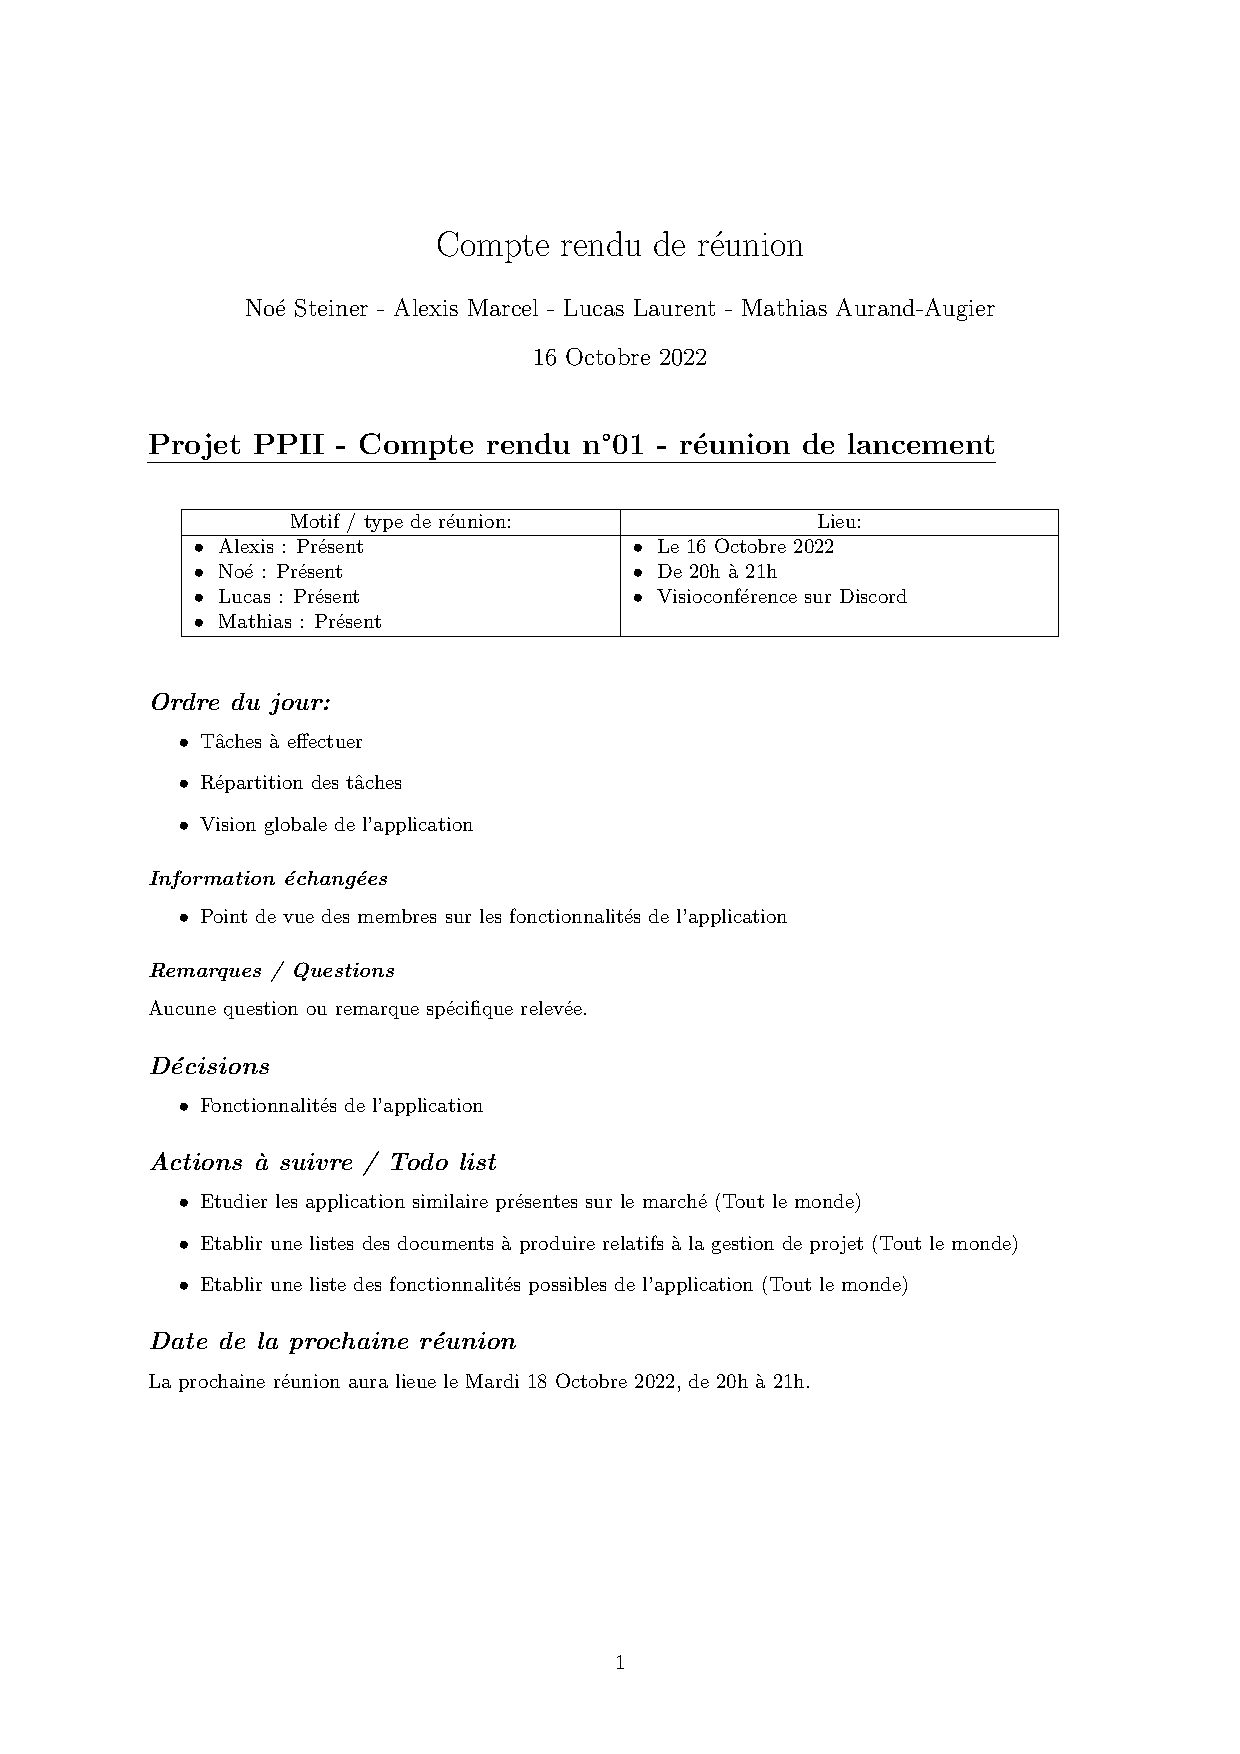
\includepdf[pages=1]{../../cr_reu/octobre/16/cr_16_octobre.pdf}
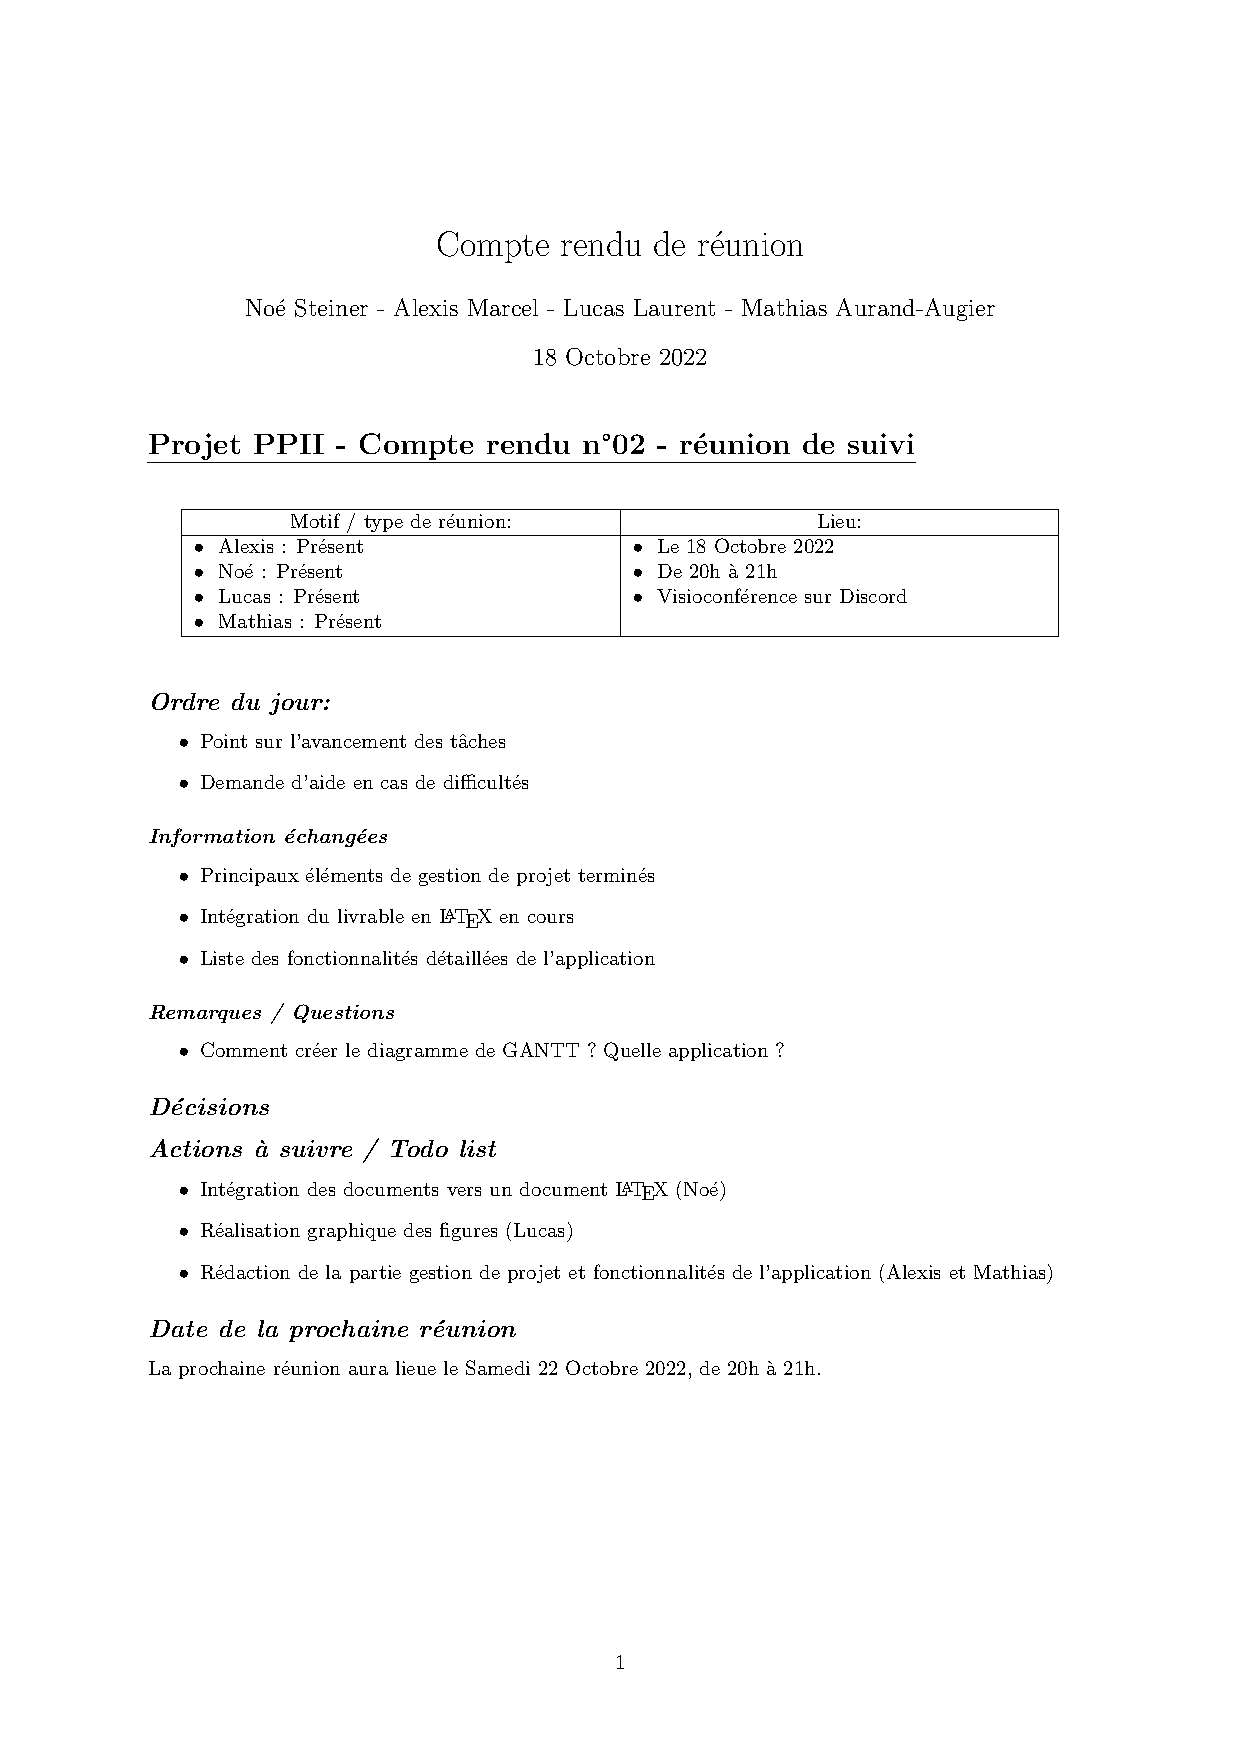
\includepdf[pages=1]{../../cr_reu/octobre/18/cr_18_octobre.pdf}
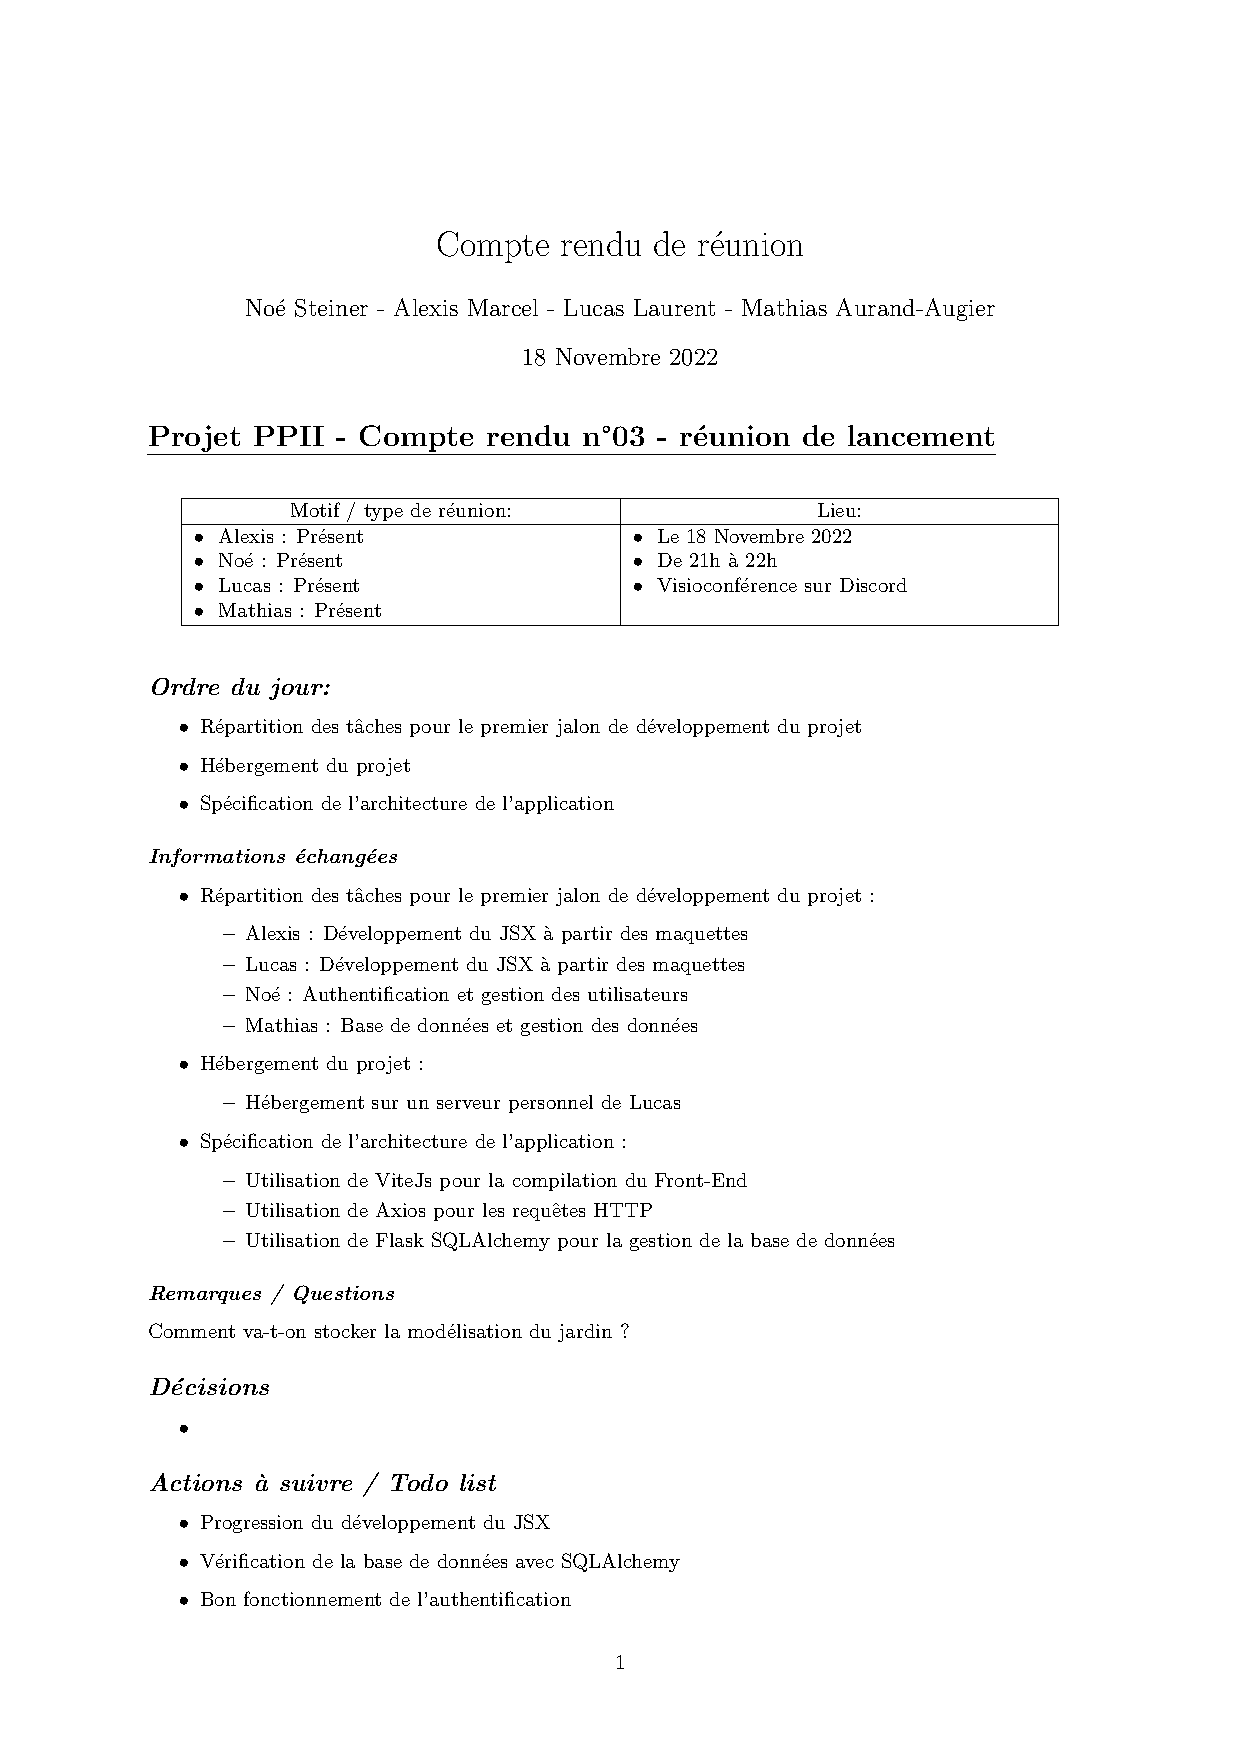
\includepdf[pages=1]{../../cr_reu/novembre/18/cr_18_novembre.pdf}
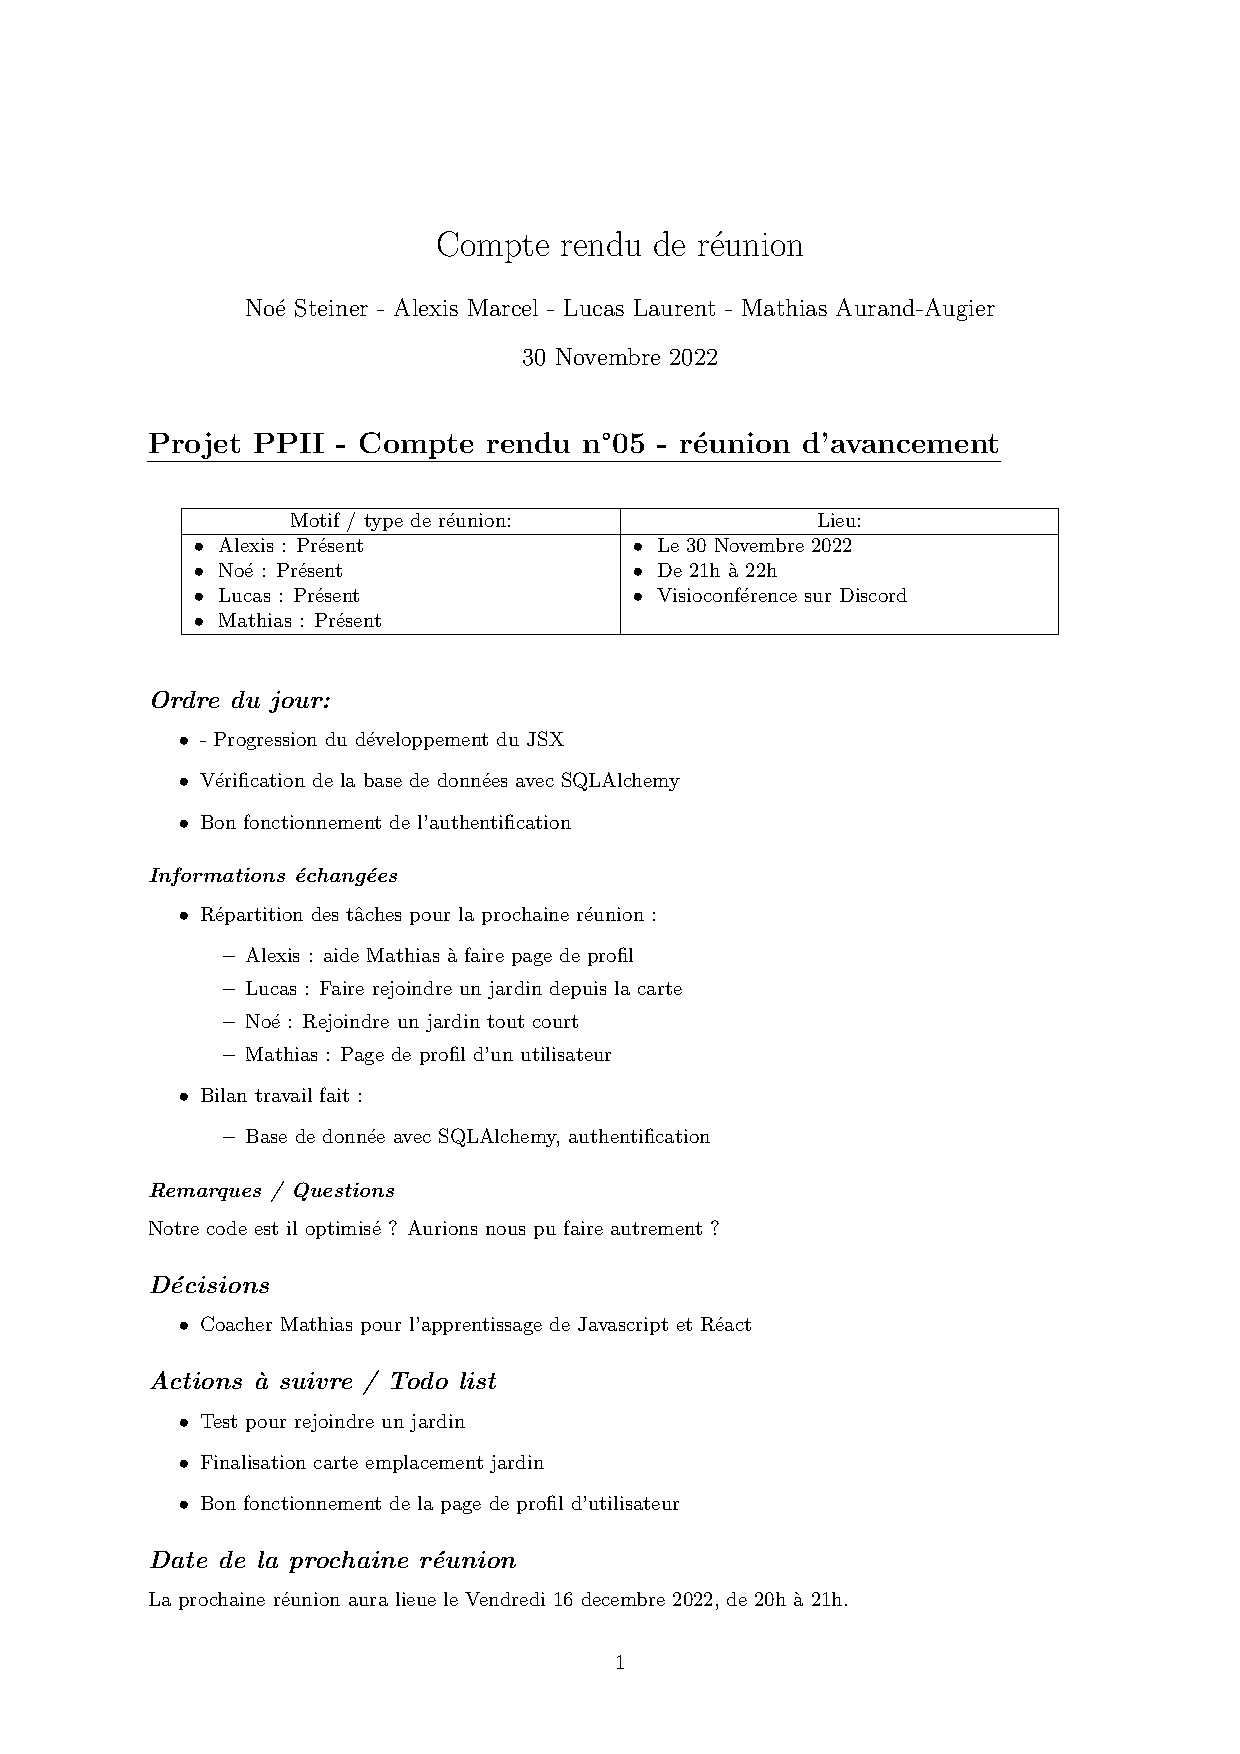
\includepdf[pages=1]{../../cr_reu/novembre/30/cr_30_novembre.pdf}
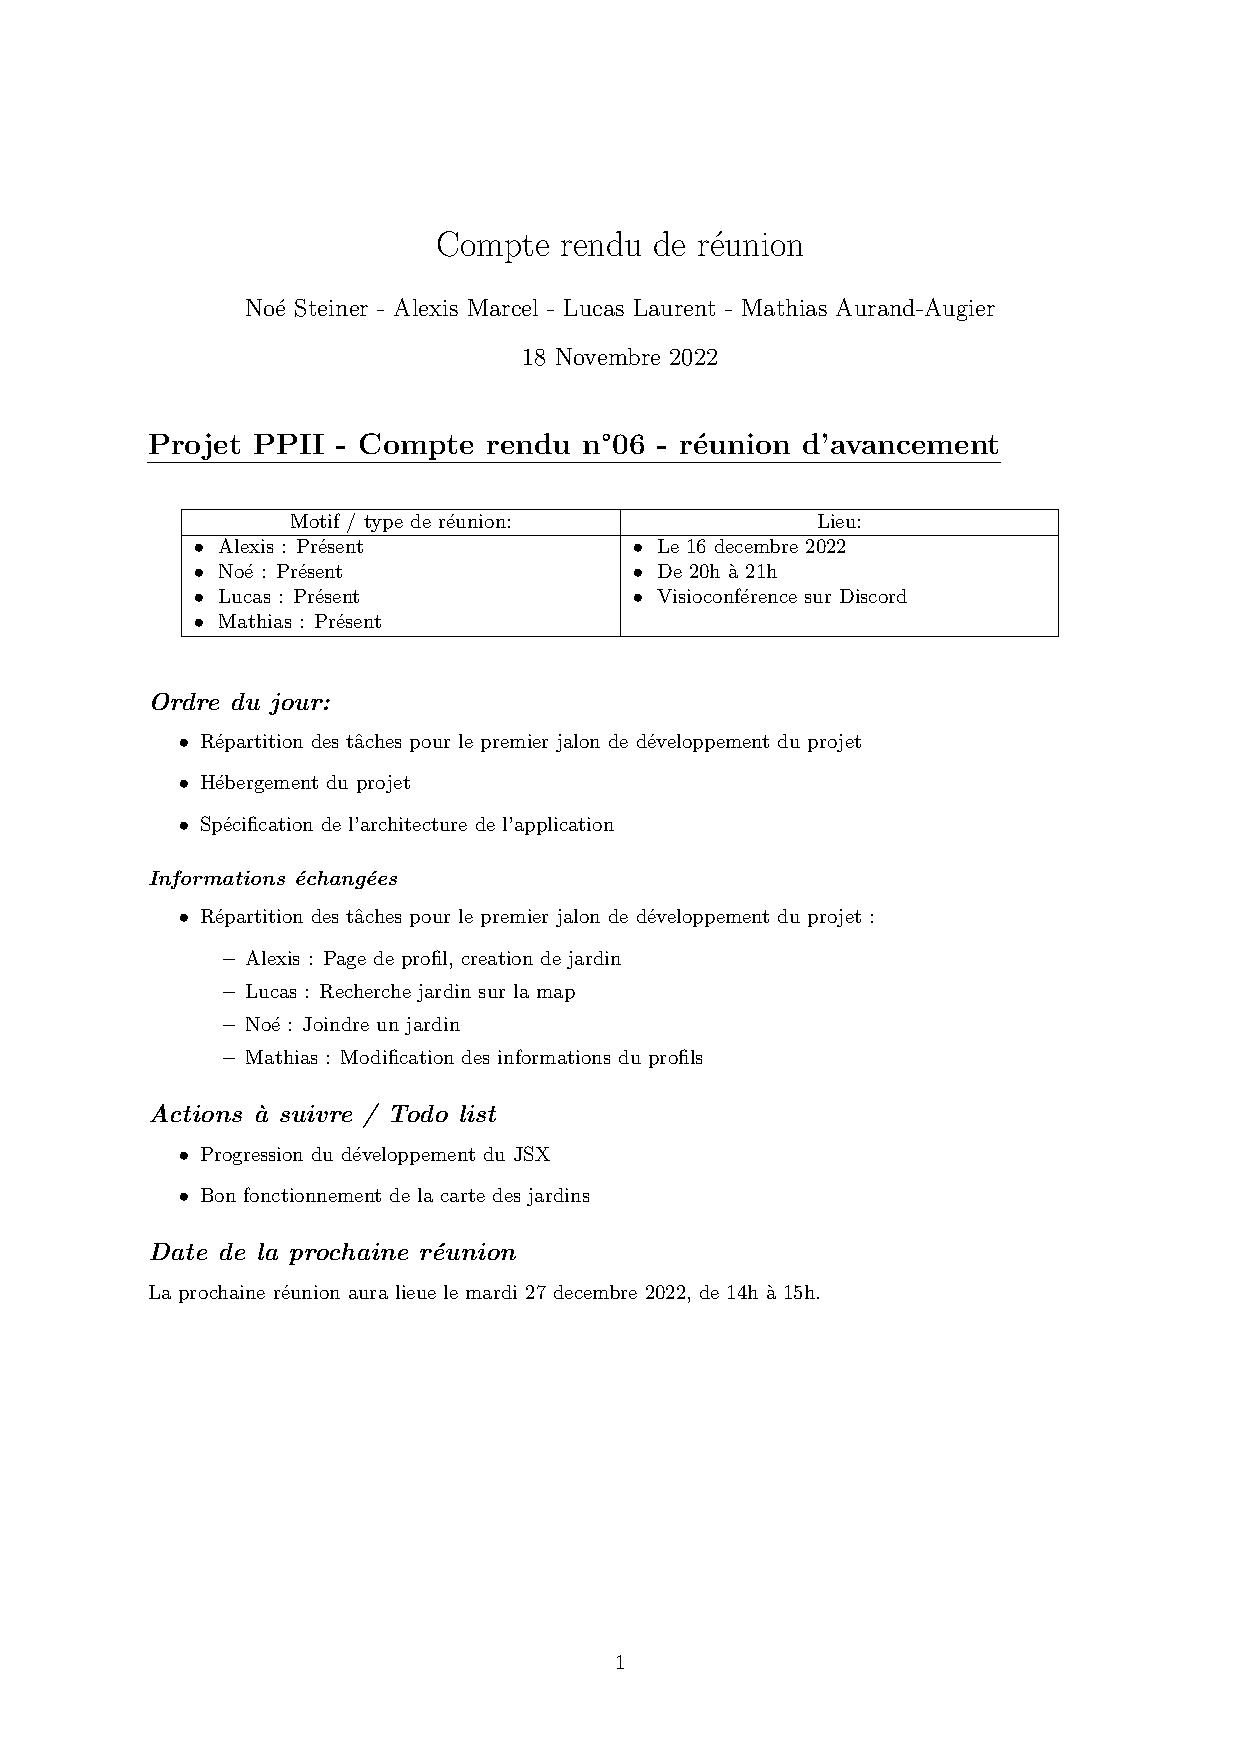
\includepdf[pages=1]{../../cr_reu/decembre/16/cr_16_decembre.pdf}
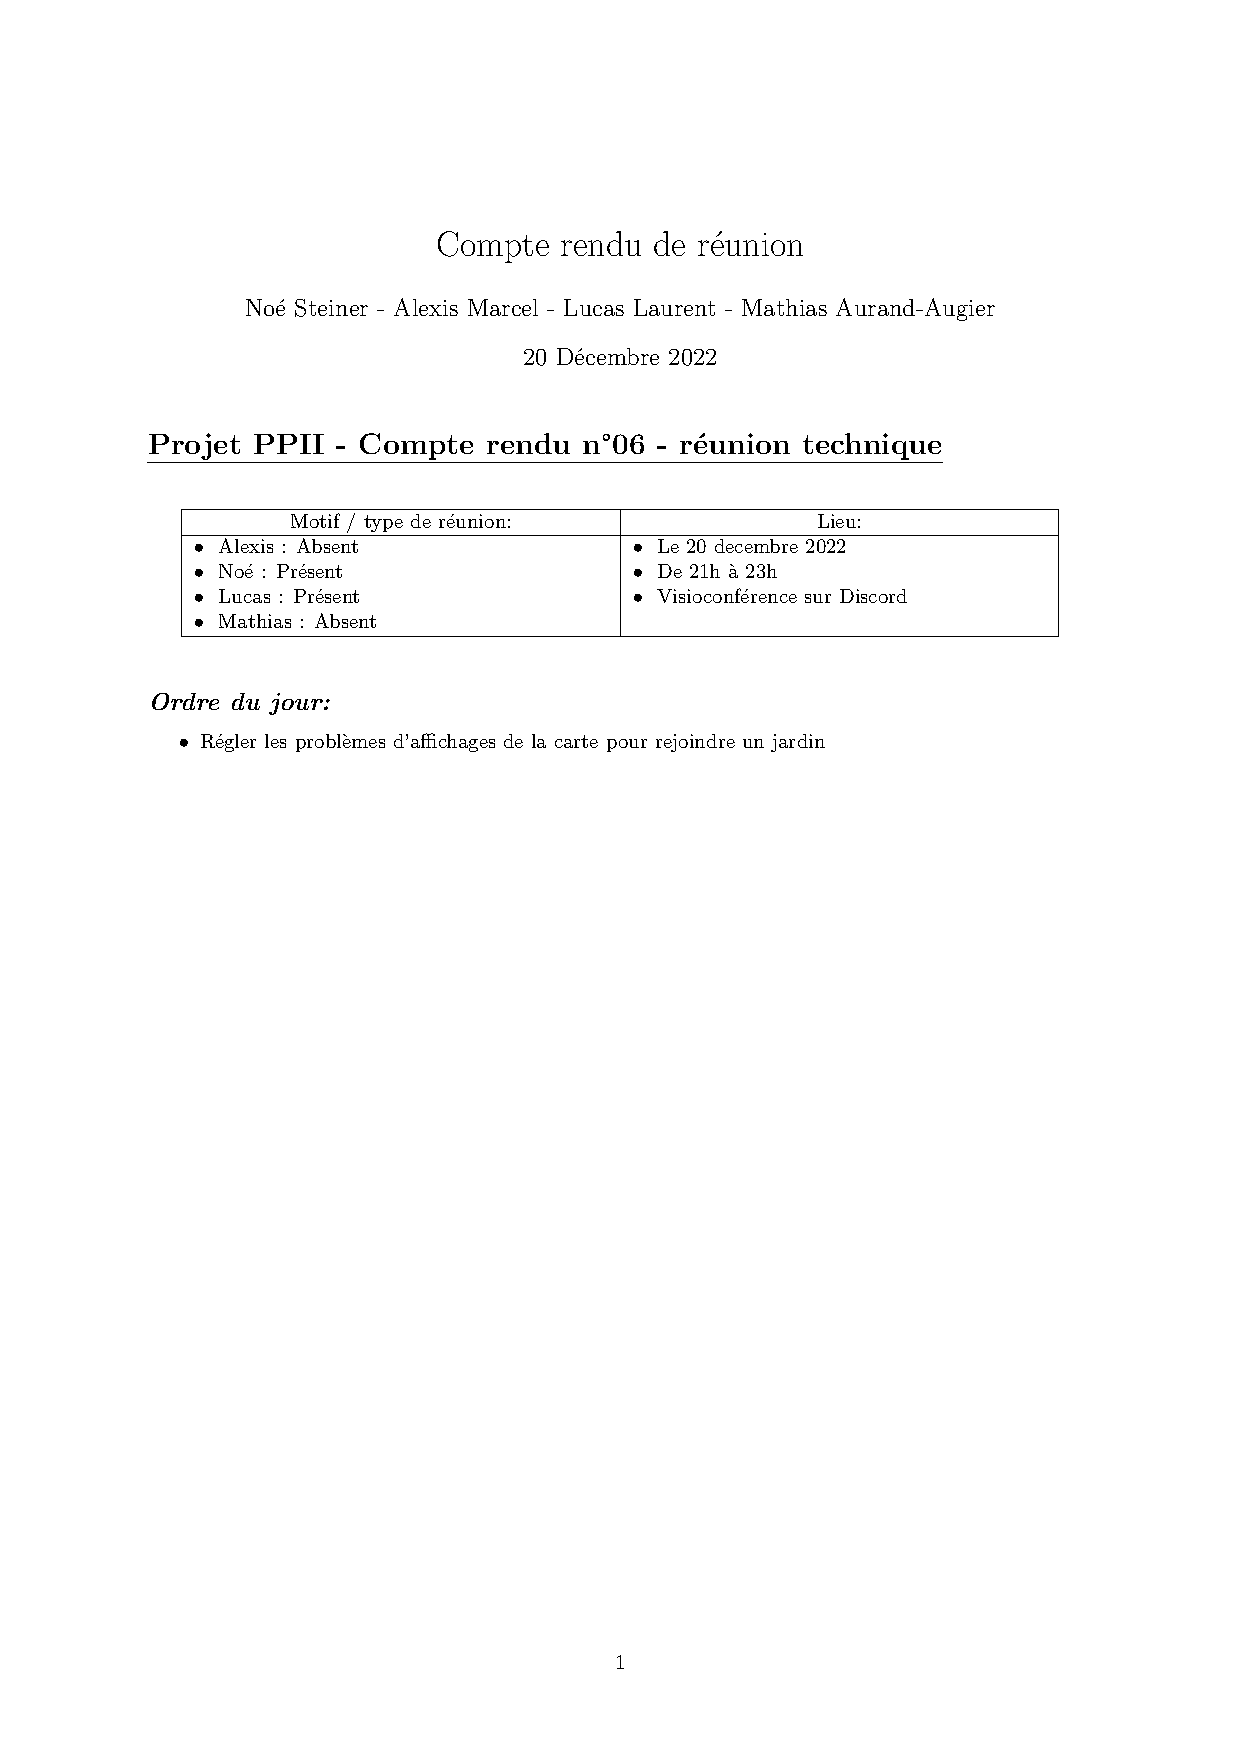
\includepdf[pages=1]{../../cr_reu/decembre/20/cr_20_decembre.pdf}
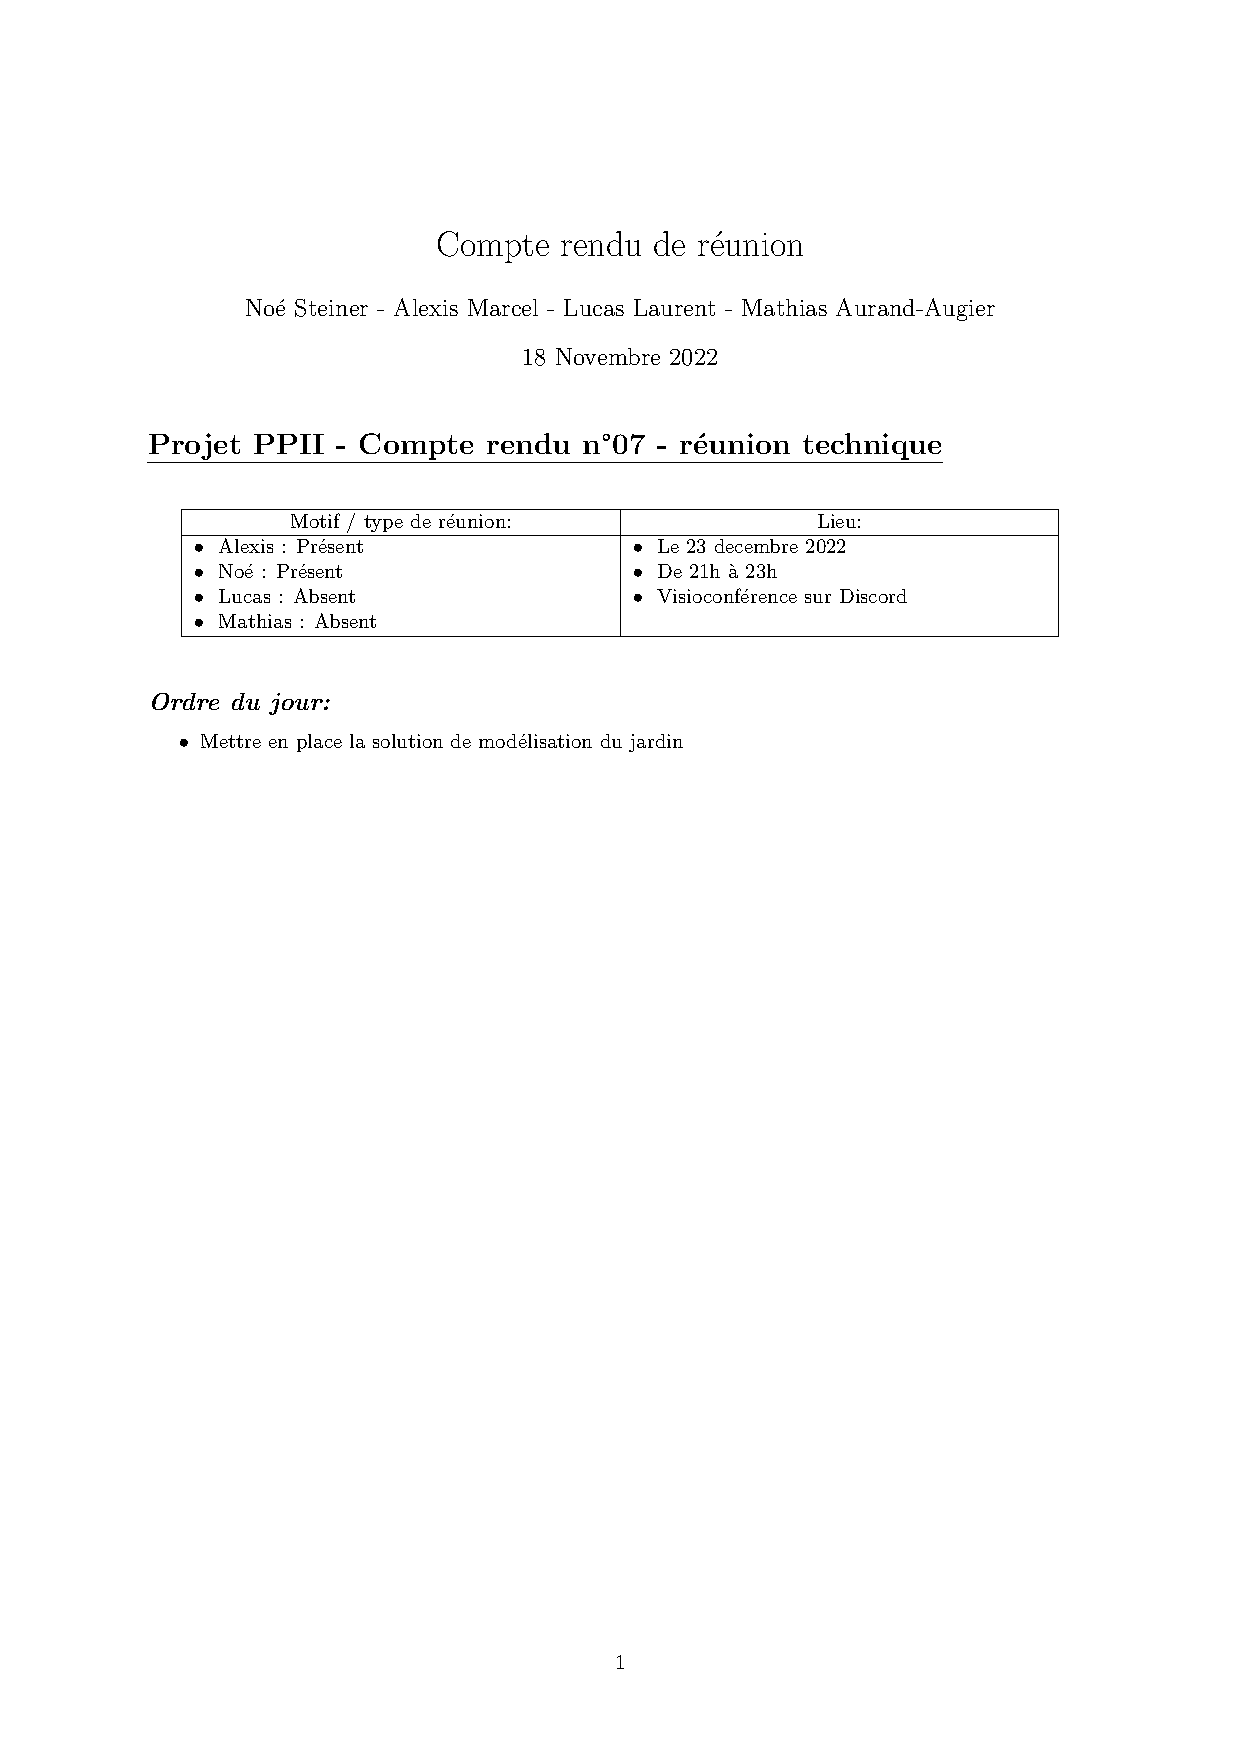
\includepdf[pages=1]{../../cr_reu/decembre/23/cr_23_decembre.pdf}
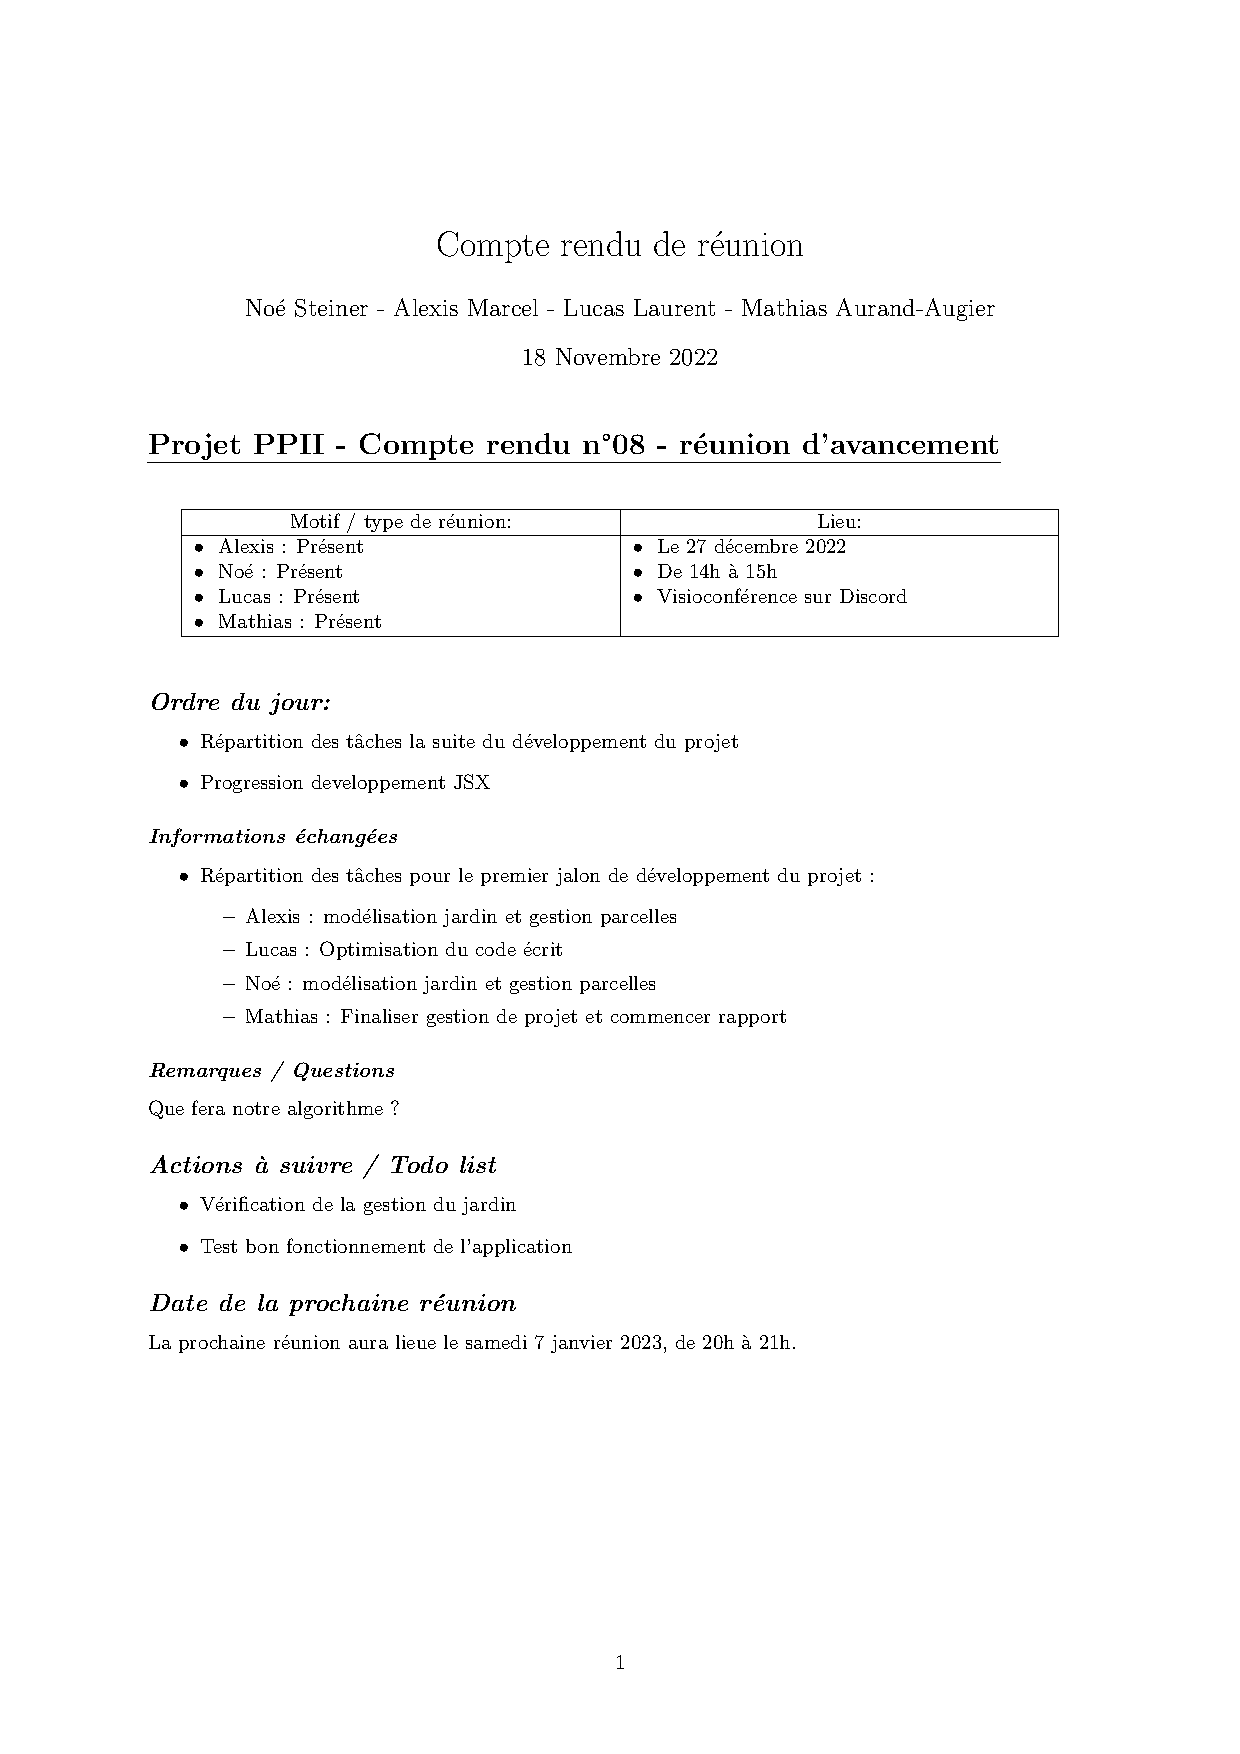
\includepdf[pages=1]{../../cr_reu/decembre/27/cr_27_decembre.pdf}
\end{document}